%%% Reset counters for the footnotes and compound numbering
%\setcounter{compound}{0}
\stepcounter{cmpreset}

\captionsetup[figure]{list=no} % hide figures from list in experimental section

\chapter{Catalysis of Etherification Reactions with sp$^3$ Electrophiles}
 %\thispagestyle{empty}
 \pagebreak
 
 \section{Introduction}
\doublespacing
 The formation of \ce{C-O} bonds through the activation of \textit{sp$^2$} hybridized electrophiles
 has been extensively studied. Catalytic methods based on
 4-(dialkylamino)pyridines proceed through a well understood nucleophilic activation mechanism.\footnote{For mechanistic studies
 see: (a) {\frenchspacing H\"ofle, G.; Steglich, W.; Vorbr\"uggen, H. 4-Dialkylaminopyridines as
 Highly Active Acylation Catalysts. \textit{Angew. Chem. Int. Ed.} \textbf{1978}, \textit{17}, 569-583.}
 (b) {\frenchspacing Spivey, A. C.; Arseniyadis, S. Nucleophilic Catalysis by
 4-(Dialkylamino)pyridines Revisited--The Search for Optimal Reactivity and Selectivity.
 \textit{Angew. Chem. Int. Ed.} \textbf{2004}, \textit{43}, 5436-5441.} (c) {\frenchspacing Held,
 I.; Villinger, A.; Zipse, H. The Stability of Acylpyridinium Cations and Their Relation to the
 Catalytic Activity of Pyridine Bases. \textit{Synthesis} \textbf{2005}, \textit{9}, 1425-1430.}
 (d) {\frenchspacing Xu, S.; Held, I.; Kempf, B.; Mayr, H.; Steglich, W.; Zipse, H. The
 DMAP-Catalyzed Acetylation of Alcohols--A Mechanistic Study. \textit{Chem. Eur. J.} \textbf{2005},
 \textit{11}, 4751-4757.} (e) {\frenchspacing Lutz, V.; Glatthaar, J.; W\"urtele, C.; Serafin, M.;
 Hausmann, H.; Schreiner, P. R. Structural Analyses of \textit{N}-Acetylated
 4-(Dimethylamino)pyridine (DMAP) Salts. \textit{Chem. Eur. J.} \textbf{2009}, \textit{15},
 8548-8557.}} A multitude of catalytic enantioselective methods have subsequently been developed
 that rely on the nucleophilic activation of \textit{sp$^2$} hybridized
 electrophiles with chiral Lewis bases.\footnote{{\frenchspacing France, S.; Guerin, D. J.; Miller,
 S.
 J.; Lectka, T.
 Nucleophilic Chiral Amines as Catalysts in Asymmetric Synthesis. \textit{Chem. Rev.} \textbf{2003},
 \textit{103}, 2985-3012.}} Among the most successful are those based on the DMAP (\ref{cmp:alkaaa})
 and PPY (\ref{cmp:alkaab}) framework introduced by the Fu\footnote{{\frenchspacing Hodous, B. L.;
 Ruble, J. C.; Fu, G.
 C. Enantioselective Addition of Alcohols to Ketenes Catalyzed by a Planar-Chiral Azaferrocene:
 Catalytic Asymmetric Synthesis of Arylpropionic Acids. \textit{J. Am. Chem. Soc.} \textbf{1999},
 \textit{121}, 2637-2638.} \label{ref:alkfu}} and Fuji\footnote{{\frenchspacing Kawabata, T.;
 Nagato, M.; Takasu, K.; Fuji, K.
 Nonenzymatic Kinetic Resolution of Racemic Alcohols through an ``Induced Fit'' Process. \textit{J.
 Am. Chem. Soc.} \textbf{1997}, \textit{119}, 3169-3170.} \label{ref:alkfuji}}
 (\refscheme{alkdmapintro}).
 The Miller group has also found success using an imidaozle ring, part of a chiral tripeptide, as
 the nucleophilic activating moiety.\footnote{{\frenchspacing Miller, S. J.; Copeland, G. T.;
 Papaioannou, N.; Horstmann, T. E.; Ruel, E. M. Kinetic Resolution of Alcohols Catalyzed by
 Tripeptides Containing the \textit{N}-Alkylimidazole Substructure. \textit{J. Am. Chem. Soc.}
 \textbf{1998}, \textit{120}, 1629-1630.} \label{ref:alkmiller}}
 
 
 With the exception of soluble iodide sources such as TBAI,
 catalytic nucleophilic activation of \textit{sp$^3$} hybridized electrophiles remains a largely
 undeveloped area.\footnote{For examples of TBAI in homogeneous alkylation reactions see: (a) {\frenchspacing Kanai, K.; Sakamoto, I.; Ogawa, S.; Suami, T.
 Synthesis on 1,4-Diaminocyclitol Antibiotics. III. Synthesis of 4-Hydroxypurpurosamine B Derivatives. \textit{Bull. Chem. Soc. Jpn.} \textbf{1987}, \textit{60},
 1529-1531.} (b) {\frenchspacing Nemoto, H.; Takamatsu, S.; Yamamoto, Y.
 An Improved and Practical Method for the Synthesis of Optically Active Diethyl Tartrate Dibenzyl Ether. \textit{J.
 Org. Chem.} \textbf{1991}, \textit{56}, 1321-1322.}} In biological settings, \textit{S}-adenosyl methionine (SAM) serves as an activator for the methyl
 group by forming an intermediate sulfonium species.\footnote{{\frenchspacing Roje, S.
 \textit{S}-Adenosyl-L-methionine:
 Beyond the Universal Methyl Group Donor. \textit{Phytochem.} \textbf{2006}, \textit{67},
 1686-1698.}} To the best of our knowledge, there are no
 examples of catalytic activation of \textit{sp$^3$} electrophiles with Lewis basic small organic
 molecules for \ce{C-O} bond forming reactions.\footnote{A singular example was found where 
 catalytic dimethylsulfide was used with \ce{Ag2O} to enhance the yield of methyl ether formation.
 No discussion of mechanism was provided. {\frenchspacing Werz, D.
 B.; Seeberger, P. H. Total Synthesis of Antigen Bacillus Anthracis Tetrasaccharide--Creation of an Anthrax
 Vaccine Candidate. \textit{Angew. Chem. Int. Ed.} \textbf{2005}, \textit{44}, 6315-6318.}
 \label{ref:alkpossiblecat}} \begin{Scheme}[t]
  \centering 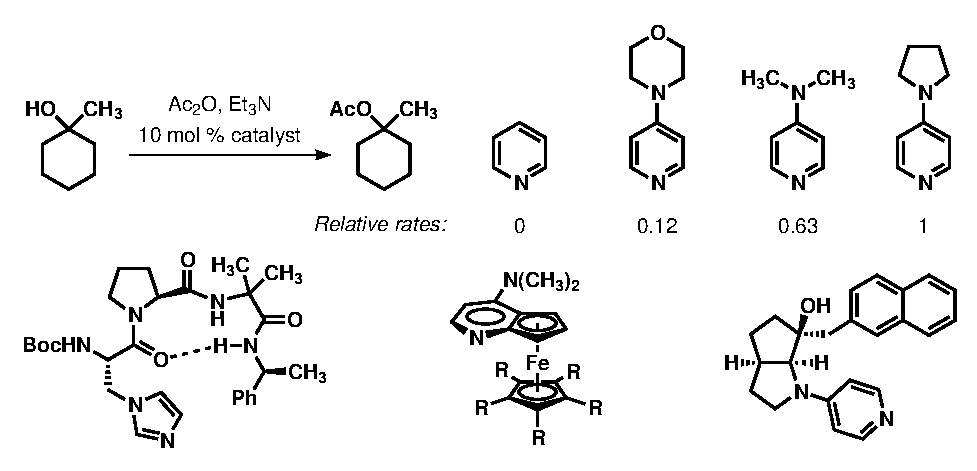
\includegraphics[scale=0.8]{chp_alkylation/images/dmapintro}
  \begin{textblock}{5}(2.3,0.4) \small \textsf{\textit{Miller}
  \textbf{1998}\crossref{ref:alkmiller}}\end{textblock}
    \begin{textblock}{5}(8,0.4) \small \textsf{\textit{Fu}
  \textbf{1999}\crossref{ref:alkfu}}\end{textblock}
    \begin{textblock}{5}(14,0.4) \small \textsf{\textit{Fuji}
  \textbf{1997}\crossref{ref:alkfuji}}\end{textblock}
  \vspace{20pt}
  \begin{textblock}{1}(14,-5.9) \cmp{alkaaa} \end{textblock}
  \begin{textblock}{1}(16.4,-5.9) \cmp{alkaab} \end{textblock}
  \caption{Nucleophilic catalysis with \textit{sp$^2$} hybridized electrophiles.}
  \label{sch:alkdmapintro}
\end{Scheme}   
 Our original intent was to find a suitable nucleophilic activator for
 electrophiles with leaving groups attached directly to \textit{sp$^3$} hybridized carbons.
 Discovery of a small molecule catalyst capable of generating more reactive \textit{sp$^3$}
 electrophiles \textit{in situ}, and possibly even chiral electrophiles from achiral or racemic
 precursors, could have a broad impact on synthetic chemistry. In the ideal reaction, carbon, nitrogen, oxgen, and other atoms
 could serve as potential nucleophiles, allowing formation of \ce{C-C}, \ce{C-N}, and \ce{C-O}
 bonds (\refscheme{alkidealreaction}).
 \begin{Scheme}[h]
  \centering \includegraphics[scale=0.8]{chp_alkylation/images/idealreaction}
  \caption{Hypothetical activation of \textit{sp$^3$} hybridized electrophiles for alkylation
  reactions.}
  \label{sch:alkidealreaction}
\end{Scheme} 
 
 \pagebreak
 \section{Discovery of a Catalyzed Reaction}
 \subsection{Initial Lewis-Base Screening}

 We began by screening a number of potential Lewis basic additives against mild etherification
 conditions.\footnote{Etherification reactions are typically carried out with the more nucleophilic
 alkoxide and an alkyl halide. (a) {\frenchspacing Williamson, A. Ueber die Theorie der
 Aetherbildung.
 \textit{Liebigs Ann. Chem.} \textbf{1851}, \textit{77}, 37-49.} (b) Feuer, H.; Hooz, J. Methods of Formation of
 the Ether Linkage. In \textit{The Chemistry of the Hydroxyl Group}; Patai, S., Ed.; Wiley: New
 York, 1967; pp 445-498.} In THF as solvent with a variety of weak bases (DIPEA, TMG, \ce{K2CO3}) to
 help scavenge the equivlent of HX produced, conversion to the target ether was never observed,
 even at elevated temperatures (\refscheme{alkinitiallewisbasescreen}). Alkylation of either the
 base or the additive was consistent with the formation of a precipitate in most cases, and the
 salts formed were not competent electrophiles.\footnote{An experiment with stoichiometric
 commercial trimethylsulfonium iodide did not show any methyl ether formation.} \begin{Scheme}[h]
 \centering
 \includegraphics[scale=0.8]{chp_alkylation/images/initiallewisbasescreen}
 \begin{textblock}{1}(3.35,-9) \cmp{alkaac} \end{textblock}
  \caption{Initial screening of Lewis bases affords no product in every case.}
  \label{sch:alkinitiallewisbasescreen}
\end{Scheme} 
 A screen of solvents (toluene, \ce{CH2Cl2}, DMF, \ce{CH3CN}) also did not lead to any productive
 reaction under the conditions tested. The use of stronger bases such as NaH or KH formed a much
 more reactive alkoxide nucleophile and even at low temperatures reactions proceeded rapidly to
 complete conversion without additives, leaving little room for catalysis. 
 
 When stoichiometric \ce{Ag2O} was employed as the base, a moderate increase in conversion
 was observed with catalytic dimethylsulfide or triphenylphosphine oxide present in the
 reaction mixture
 (\ref{cmp:alkaac}\ce{->}\ref{cmp:alkaad},
 \refscheme{alksilverscreen}).\crossref{ref:alkpossiblecat} The use of
 \ce{Ag2O} helps activate the electrophile by generating a highly insoluble silver halide
 salt, essentially functioning as a halide-specific Lewis acid.\footnote{For recent examples of
 alkylation reactions assisted by \ce{Ag2O} see:
 (a) {\frenchspacing Gouliaras, C.; Lee, D.; Chan, L.; Taylor, M. S. Regioselective Activation of Glycosyl Acceptors by a Diarylborinic Acid-Derived Catalyst. \textit{J. Am. Chem. Soc.}
\textbf{2011}, \textit{133}, 13926-13929.} (b) {\frenchspacing Chan, L.; Taylor, M. S.
Regioselective Alkylation of Carbohydrate Derivatives Catalyzed by a Diarylborinic Acid Derivative.
\textit{Org. Lett.} \textbf{2011}, \textit{13}, 3090-3093.}} The presence of sulfur or phosphine
oxide additives could potentially serve as silver(I) ligands, producing a more soluble silver
salt.\footnote{{\frenchspacing Daubinet, A. Design, Synthesis and Evaluation of Silver-Specific
Ligands.
Ph.D.
Dissertation, Rhodes University, Grahamstown, South Africa, 2001.}} This may explain why we observed
a subtle increase in conversion. We were wary of developing a reaction with
stoichiometric silver, and also had concerns that the additive was not actually functioning as a
nucleophilic activator. 
\begin{Scheme}[h]
\centering
 \includegraphics[scale=0.8]{chp_alkylation/images/silverscreen}
 \begin{textblock}{1}(3.6,-0.4) \crossrefcmp{alkaac} \end{textblock}
 \begin{textblock}{1}(9.7,-0.4) \cmp{alkaad} \end{textblock}
  \caption{Moderate conversion increase with dimethyl sulfide and triphenylphosphine oxide.}
  \label{sch:alksilverscreen}
\end{Scheme} 

 \subsection{Discovery of Imidazolium Salt Catalyzed Reactions}
 
  \begin{Scheme}[p] \centering
 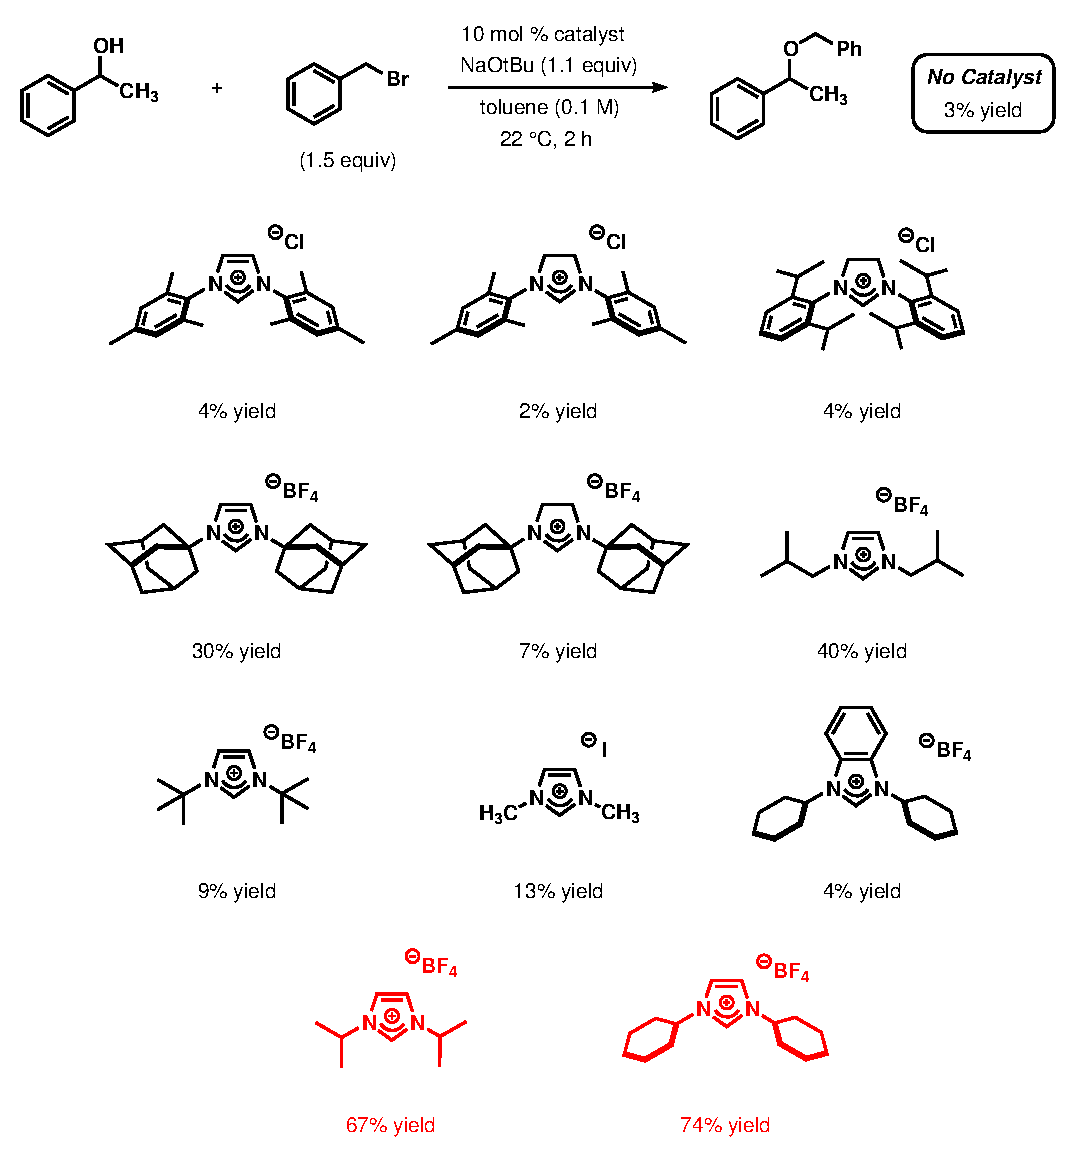
\includegraphics[scale=0.8]{chp_alkylation/images/imidazoliumscreen}
 \begin{textblock}{1}(1.7,-17.7) \crossrefcmp{alkaac} \end{textblock}
  \begin{textblock}{1}(14.3,-17.7) \cmp{xcaa} \end{textblock}
 %%% row 1
 \begin{textblock}{1}(4.1,-13.8) \cmp{alkaae} \end{textblock}
 \begin{textblock}{1}(9.9,-13.8) \cmp{alkaaf} \end{textblock}
 \begin{textblock}{1}(15.2,-13.8) \cmp{alkaag} \end{textblock}
 %%% row 2
 \begin{textblock}{1}(4.1,-9.5) \cmp{alkaah} \end{textblock}
 \begin{textblock}{1}(9.8,-9.5) \cmp{alkaai} \end{textblock}
 \begin{textblock}{1}(15.2,-9.5) \cmp{alkaaj} \end{textblock}
 %%% row 3
 \begin{textblock}{1}(4.1,-5.2) \cmp{alkaak} \end{textblock}
 \begin{textblock}{1}(9.8,-5.2) \cmp{alkaal} \end{textblock}
 \begin{textblock}{1}(15.2,-5.2) \cmp{alkaam} \end{textblock}
 %%% row 4
 \begin{textblock}{1}(6.8,-1) \cmp{alkaan} \end{textblock}
 \begin{textblock}{1}(12.8,-1) \cmp{alkaao} \end{textblock}
 
 \vspace{15pt}
  \caption{Screen of imidazolium and imidazolinium salts for catalytic activity.}
  \label{sch:alkimidazoliumscreen}
\end{Scheme} 
 After looking at standard nitrogen, oxygen, sulfur, selenium, and phosphorus centered Lewis
 bases and failing to observe any serious catalysis, we decided to examine carbon centered \textit{N}-hetereocyclic carbenes. In the presence of a suitable base, imidazolium and imidazolinium salts
 could be deprotonated to furnish the NHC.\footnote{(a) {\frenchspacing Sch\"onherr, H. J.; Wanzlick, H. W.
 Chemie Nucleophiler Carbene, XVIII. 1,3,4,5-Tetraphenyl-imidazoliumperchlorat. \textit{Liebigs Ann.
 Chem.} \textbf{1970}, \textit{731}, 176-179.} (b) {\frenchspacing Arduengo, A. J.; Harlow, R. L.;
 Kline, M. A Stable Crystalline Carbene. \textit{J. Am. Chem. Soc.} \textbf{1991}, \textit{113},
 361-363.} (c) {\frenchspacing Arduengo, A. J.; Dias, H. V. R.; Harlow, R. L.; Kline, M. Electronic
 Stabilization of Nucleophilic Carbenes. \textit{J. Am. Chem. Soc.} \textbf{1992}, \textit{114},
 5530-5534.}} We began by screening a variety of sterically and electronically differentiated
 commercially available imidazolium and imidazolinium salts (\refscheme{alkimidazoliumscreen}). When
 1-phenylethanol (\ref{cmp:alkaac}) was subjected to benzyl bromide and sodium
 \textit{tert}-butoxide in toluene as solvent, after two hours a 3\% yield of the target ether
 \ref{cmp:xcaa} was observed by $^1$H NMR. Salts bearing sterically hindered aryl groups
 (\ref{cmp:alkaae}, \ref{cmp:alkaaf}, and \ref{cmp:alkaag}) did not appear to provide any additional
 product. We were exceptionally pleased to see a 30\% yield with bis-adamantyl imidazolium
 \ref{cmp:alkaah}, a ten-fold increase in yield over the uncatalyzed reaction. The corresponding
 imidazolinium salt \ref{cmp:alkaai} delivered a marginal 7\% yield. The yield again increased to
 40\% with isobutyl substituted imidazolium \ref{cmp:alkaaj}. The bis-\textit{tert}-butyl
 (\ref{cmp:alkaak}) and bis-methyl (\ref{cmp:alkaal}) imidazolium salts were ineffective.
 Benzimidazolium \ref{cmp:alkaam} also provided no advantage over the uncatalyzed background
 reaction. The highest yields were obtained with bis-isopropyl imidazolium \ref{cmp:alkaan} (67\%)
 and bis-cyclohexyl imidazolium \ref{cmp:alkaao} (74\%). These data suggested that an unsaturated
 imidazolium ring and a secondary \textit{sp$^3$} hybridized carbon attached to the nitrogens were
 key structural features.
 

 \begin{Scheme}[h]
 \centering
 \includegraphics[scale=0.8]{chp_alkylation/images/saltcontrols}
 \begin{textblock}{1}(1.7,-2.9) \crossrefcmp{alkaac} \end{textblock}
  \begin{textblock}{1}(9.5,-2.9) \crossrefcmp{xcaa} \end{textblock}
  \begin{textblock}{1}(1.8,-0.4) \cmp{alkaap} \end{textblock}
    \begin{textblock}{1}(14.5,-1.2) \cmp{alkaaq} \end{textblock}
      \begin{textblock}{1}(18.3,-1.2) \cmp{alkaar} \end{textblock}
  \caption{Control reactions establish requirement of the imdazolium ring for catalysis.}
  \label{sch:alksaltcontrols}
\end{Scheme} 
 In order to establish that the imidazolium salt was in fact necessary for catalysis, we ran a
 series of control experiments (\refscheme{alksaltcontrols}). With sodium tetrafluoroborate or
 tetramethylphosphonium bromide present, less than 5\% yield of the product was observed. Other
 cationic heterocylic salts derived from 2,6-lutidine (\ref{cmp:alkaaq} and
 \ref{cmp:alkaar}) did not accelerate the reaction. Starting from the sodium alkoxide
 \ref{cmp:alkaap},\footnote{Formed by deprotonation of \ref{cmp:alkaac} with NaH in THF inside an inert atmosphere glovebox. The $\Delta\delta$
 ($\delta$\ref{cmp:alkaap}$-\delta$\ref{cmp:alkaac}) of the benzyllic methine proton by $^1$H NMR in
 toluene-\textit{d}$_8$ was $+$0.17 ppm after concentration and trituration with
 toluene.} which was fully soluble in toluene, a slightly higher 10\% yield was obtained in the
 absence of any catalyst.
 This result indicates that \textit{tert}-butanol present in the reaction mixture had a subtle
 inhibitory effect, presumably through hydrogen bonding to the nucleophile. These control reactions
 suggest that the nitrogen hetereocyclic plays a critical role in the reaction. Specifically,
 imidazolium heterocycles bearing the appropriate alkyl substituents were required to obtain any catalytic activity.
 

\pagebreak

 \section{Mechanistic Studies}
  In the sections that follow, a discussion of the mechanism of this transformation will be
 presented. Several hypotheses were proposed and rigorously tested before finally arriving at a
 mechanism we believed to be consistent with the complete set of data. 
 
 
 \subsection{Preliminary Hypothesis Based on Electrophile Activation}
 Crystallographic evidence from the literature suggested that carbenes were capable of
 reacting as nucleophiles with various \textit{sp$^3$} hybridized electrophiles
 (\reffigure{alkknappkecrystals}).\footnote{(a) {\frenchspacing Knappke, C.
 E.
 I.; Neud\"orfl, J. M.; von Wangelin, A. J. On New N-Heterocyclic Carbene Derived Alkylidene
 Imidazolines.
 \textit{Org. Biomol. Chem.} \textbf{2010}, \textit{8}, 1695-1705.} (b) {\frenchspacing Knappke, C.
 E. I.; Arduengo, A. J.; Jiao, H.; Neud\"orfl, J. M.; von Wangelin, A. J. On the Dual Role of
 \textit{N}-Heterocyclic Carbenes as Bases and Nucleophiles in Reactions with Organic Halides.
 \textit{Synthesis} \textbf{2011}, 3784-3795.} \label{ref:alkwangelin}} In 2010 and 2011 von
 Wangelin and coworkers treated aryl substituted imidazolium salts with potassium
 \textit{tert}-butoxide in THF solutions, forming the carbene, and then subsequently added various
 halide electrophiles. With an excess of base present ($>$2 equivalents), the products isolated resembled a
 deoxy Breslow intermediate,\footnote{(a) {\frenchspacing Breslow, R. On the Mechanism of Thiamine Action.
IV. Evidence from Studies on Model Systems. \textit{J. Am. Chem. Soc.} \textbf{1958}, \textit{80},
3719-3726.} (b) A Breslow intermediate was recently isolated: {\frenchspacing Berkessel, A.;
Elfert, S.; Yatham, V.
R.; Neud\"orfl, J.
M.; Schl\"orer, N. E.; Teles, J. H. Umpolung by N-Heterocyclic Carbenes: Generation and Reactivity of
the Elusive 2,2-Diamino Enols (Breslow Intermediates). \textit{Angew. Chem. Int. Ed.} \textbf{2012},
\textit{51}, 12370-12374.}} formed by alkylation at the C2 position of the imidazole ring followed
by further deprotonation at the benzylic position (\ref{cmp:alkaat}, right). The newly formed
double bond showed a length of 1.39 \AA\  in structure \ref{cmp:alkaat}, considerably longer than
the average C$_{sp^2}$\ce{=}C$_{sp^2}$ bond length (1.32 \AA),\footnote{{\frenchspacing Allen, F.
H.; Kennard, O.; Watson, D. G.; Brammer, L.; Orpen, A.
G.; Taylor, R. Tables of Bond Lengths Determined by X-ray and Neutron Diffraction. Part 1. Bond Lengths
in Organic Compounds. \textit{J. Chem. Soc. Perk. T. 2} \textbf{1987}, S1-S19.}} suggesting the bond
contains significant charge-separated ylide character. The nucleophilic nature of the benzylic
position was confirmed by adding a second equivalent of electrophile, producing doubly alkylated
imidazolium salts (not shown). This type of reactivity mirrors that observed for Breslow
intermediates in Stetter and benzoin condensation reactions.\footnote{For a lead
reference see: {\frenchspacing Enders, D.; Balensiefer, T. Nucleophilic Carbenes in Asymmetric
Organocatalysis. \textit{Acc. Chem. Res.} \textbf{2004}, \textit{37}, 534-541.}} The protonated imidazolium salt
\ref{cmp:alkaas} (left) was obtained by adding TMSI to a solution containing residual
\textit{tert}-butanol from the carbene formation, liberating an equivalent of HI. Direct isolation
of \ref{cmp:alkaas} was complicated by the tendency to rapidly become deprotonated, necessitating an
acidic quench after formation of the alkylated species. 

\begin{figure}[t]
 \centering
 \vspace{2.8in}
  \begin{textblock}{1}(-0.8,-10)
   \includegraphics[scale=0.35]{chp_alkylation/images/knappke_ptol}\end{textblock}
    \begin{textblock}{1}(10,-9.5)
   \includegraphics[scale=0.35, angle=90]{chp_alkylation/images/knappke_pno2}\end{textblock}
 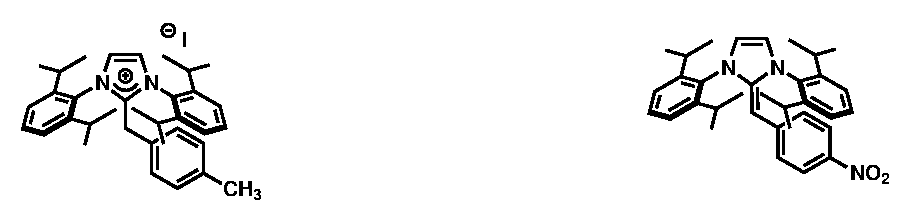
\includegraphics[scale=0.8]{chp_alkylation/images/knappkecrystals}
 \begin{textblock}{1}(3,-0.5) \cmp{alkaas} \end{textblock}
 \begin{textblock}{1}(14.3,-1) \cmp{alkaat} \end{textblock}
 \vspace{25pt}
   \begin{textblock}{5}(1.9,-0.8) \small \textsf{\textit{von Wangelin}
  \textbf{2010}\crossref{ref:alkwangelin}\textsuperscript{a}}\end{textblock}
    \begin{textblock}{5}(13,-0.8) \small \textsf{\textit{von Wangelin}
  \textbf{2011}\crossref{ref:alkwangelin}\textsuperscript{b}}\end{textblock}
  \caption{Crystal structures of products from carbenes and \textit{sp$^3$}
  electrophiles.}
  \label{fig:alkknappkecrystals}
\end{figure} 

We had hoped that in the presence of a suitable nucleophile, an
intermediate akin to \ref{cmp:alkaas} could serve as an activated electrophile. Given the precedents
for carbenes to act as nucleophiles towards \textit{sp$^3$} electrophiles, we proposed the catalytic
cycle illustrated in \refscheme{alkactivationcycleone}. Stirring the imidazolium
salt \ref{cmp:alkaao} in toluene with sodium \textit{tert}-butoxide produces the carbene
(\ref{cmp:alkaao}\ce{->i}), entering the catalytic cycle. Addition of benzyl bromide forms the
activated electrophile (\textit{i}\ce{->}\textit{ii}), which can then either directly undergo
alkylation and regenerate the carbene (\textit{ii}\ce{->}\textit{i}), or become deprotonated
(\textit{ii}\ce{->}\textit{iii}) to form a species similar to \ref{cmp:alkaat}. Reprotonation from
from the secondary alcohol would generate an imidazolium alkoxide salt pair
(\textit{iii}\ce{->}\textit{iv}). The more nucleophilic alkoxide could then attack the activated
benzyl bromide, generating the ether product and releasing the carbene for further turnovers.  Prior to the addition of the electrophile, we observed the
formation of a purple solution (top right), likely indicating formation of the
carbene.\footnote{Non-transition metal carbene complexes are known to form colored solutions. (a)
{\frenchspacing Arnold, P. L.; Rodden, M.; Wilson, C. Thermally Stable Potassium
\textit{N}-Heterocyclic Carbene Complexes with Alkoxide Ligands, and a Polymeric Crystal Structure
with Distorted, Bridging Carbenes. \textit{Chem. Commun.} \textbf{2005}, 1743-1745.} (b)
{\frenchspacing Willans, C. E. Non-transition Metal \textit{N}-Heterocyclic Carbene Complexes.
\textit{Organomet. Chem.} \textbf{2010}, \textit{36}, 1-28.}} Upon addition of benzyl bromide to the carbene solution we \textit{immediately} observed the formation of a turbid bright yellow suspension (bottom right). We believed this was consistent with the formation of intermediate \textit{iii} and the precipitation of sodium bromide.

 \begin{Scheme}[t]
 \begin{textblock}{1}(3.5,0.5) \crossrefcmp{alkaao} \end{textblock}
  \begin{textblock}{1}(11,0.5) \includegraphics[scale=0.13]{chp_alkylation/images/reactionpurple}
 \end{textblock}
 \begin{textblock}{1}(11,6.5) \includegraphics[scale=0.13]{chp_alkylation/images/reactionyellow}
 \end{textblock}
 \begin{textblock}{5}(16,2.8) \footnotesize \textsf{\ref{cmp:alkaao} $+$ NaOtBu}\end{textblock}
 \begin{textblock}{5}(16,8.8) \footnotesize \textsf{\ref{cmp:alkaao} $+$ NaOtBu $+$
 BnBr}\end{textblock}
 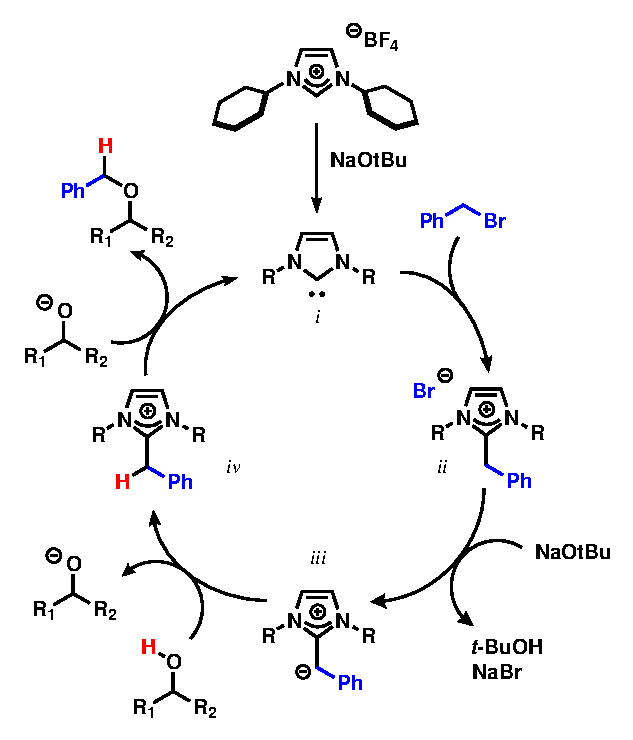
\includegraphics[scale=0.8]{chp_alkylation/images/activationcycleone}
  \caption{First mechanistic proposal involving NHC activation of the electrophile.}
  \label{sch:alkactivationcycleone}
\end{Scheme}

In order to test this mechanistic hypothesis, we designed a series of deuterium labeling
experiments. To probe for the formation of intermediate \textit{iii} in the catalytic cyle, we ran
an experiment with \textit{d$_2$}-benzyl bromide (\ref{cmp:xcap}, \refscheme{alkdeprotonationexp}).
Our expectation was that if \textit{iii} was part of the productive catalytic cycle, we would see proton incorporation into the
ether product. The recovered product \ref{cmp:xcac} showed no incorporation of protons at the
benzylic position by $^1$H NMR spectroscopy, suggesting that \textit{iii} was not part of a productive pathway in the
catalytic cycle. Regardless, the formation of \textit{iii} was not integral to this mechanism being
operative, as proposed intermediate \textit{ii} could be directly alkylated without proceeding
through intermediate \textit{iii}.

 \begin{Scheme}[t]
  \begin{textblock}{1}(1.2,2.7) \crossrefcmp{alkaac} \end{textblock}
  \begin{textblock}{1}(4.5,2.7) \cmp{xcap} \end{textblock}
  \begin{textblock}{1}(13.5,2.7) \cmp{xcac} \end{textblock}
 \includegraphics[scale=0.8]{chp_alkylation/images/deprotonationexp}
  \caption{No benzylic proton incorportation observed with \textit{d$_2$}-benzyl bromide.}
  \label{sch:alkdeprotonationexp}
\end{Scheme}

 \begin{Scheme}[b]
  \begin{textblock}{3}(0.8,3.7) \textsf{\scriptsize{(\textit{S})-}}\crossrefcmp{alkaac}
  \end{textblock}
    \begin{textblock}{3}(3.6,3.7) \textsf{\scriptsize{(\textit{R})-}}\cmp{xcao}
  \end{textblock}
  \begin{textblock}{3}(18,1) \textsf{\scriptsize{(\textit{S,R})-}}\cmp{xcab}
  \end{textblock}
  \begin{textblock}{3}(18,3.8) \textsf{\scriptsize{(\textit{S,S})-}}\crossrefcmp{xcab}
  \end{textblock}

 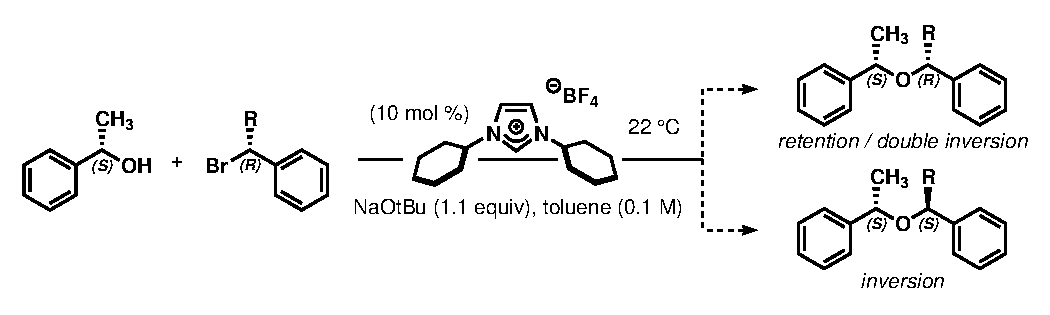
\includegraphics[scale=0.8]{chp_alkylation/images/inversionexp}
  \caption{Proposed experiment to test for nucleophilic electrophile activation.}
  \label{sch:alkinversionexp}
\end{Scheme}


We wanted to design an experiment to directly test whether or not the electrophile was being
activated through a nucleophilic displacement of the leaving group. In the proposed mechanism, the
electrophile would undergo two inversions at the site of the leaving group -- once upon addition of
the carbene (\textit{i}\ce{->}\textit{ii}) and again when the nucleophile attacks 
(\textit{iv}\ce{->}\textit{i}). Starting from a chiral optically pure alcohol and reacting that with
a chiral secondary electrophile would give different diastereomers of the product depending on the
mechanism (\refscheme{alkinversionexp}). Double inversion of the electrophile, a net retention of
the original configuration, would lead to a different diastereomer than direct S$_\mathrm{N}$2 substitution.
Alternatively, a 50:50 mixture of diastereomers would be indicative of an S$_\mathrm{N}$1 pathway.
While both (\textit{R})-- and (\textit{S})-$\alpha$-methylbenzyl bromide (R = \ce{CH3}) were known
compounds and could be readily prepared from the commercially available
chiral alcohol,\footnote{{\frenchspacing Chen, Y.; Tang, W.
L.; Mou, J.; Li, Z.
High-Throughput Method for Determining the Enantioselectivity of Enzyme-Catalyzed Hydroxylations Based on Mass Spectrometry.
\textit{Angew. Chem. Int. Ed.} \textbf{2010}, \textit{49}, 5278-5283.}} attempts to use the more
hindered secondary electrophile were unsuccessful. We decided to target \textit{d$_1$}-benzyl
bromide (R = D) and were presented with the unique challenge of preparing a stereogenic center
containing a hydrogen and deuterium.

 \begin{Scheme}[h]
   \begin{textblock}{1}(14.7,7.5) \cmp{xcaq} \end{textblock}
   \begin{textblock}{1}(17.6,0.8) \crossrefcmp{xcao} \end{textblock}
   \begin{textblock}{5}(13.2,0.25) \small \textsf{\textit{Wolfe}
  \textbf{1957}\crossref{ref:alkwolfebenzylbromide}\textsuperscript{a}}\end{textblock}
    \begin{textblock}{5}(10.2,7.5) \small \textsf{\textit{Noyori}
  \textbf{2000}\crossref{ref:alknoyoritransfer}}\end{textblock}
 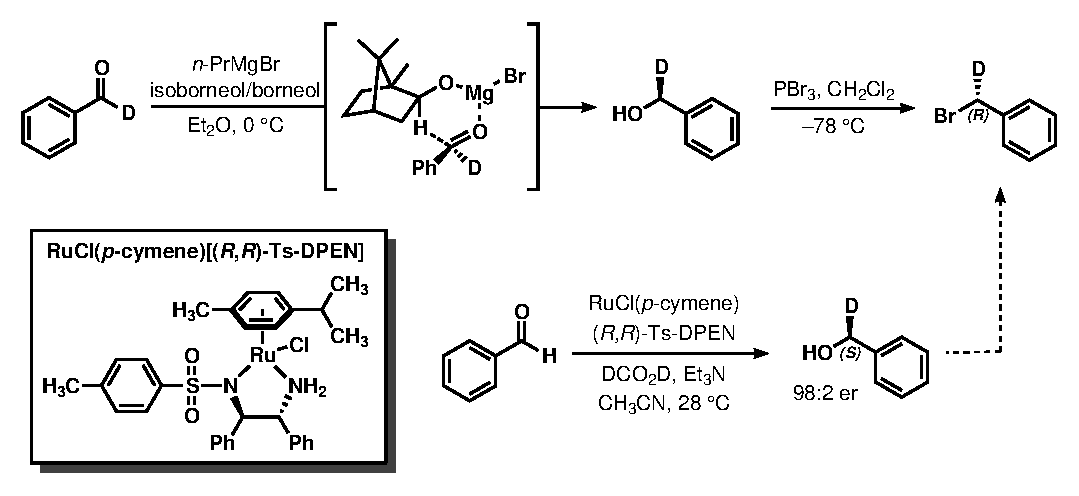
\includegraphics[scale=0.8]{chp_alkylation/images/chiralbenzylbromide}
 \vspace{5pt}
  \caption{Preparation of optically active \textit{d}$_1$-benzyl bromide.}
  \label{sch:alkchiralbenzylbromide}
\end{Scheme}
We found one early report discussing the preparation of optically active \textit{d}$_1$-benzyl
bromide (\refscheme{alkchiralbenzylbromide}, top).\footnote{(a) {\frenchspacing Streitweiser, A.;
Wolfe, J.
R.
Stereochemistry of the Primary Carbon. V. Optically Active Benzyl-$\alpha$-\textit{d} Alcohol. \textit{J. Am. Chem.
Soc.} \textbf{1957}, \textit{79}, 903-907.} (b) {\frenchspacing Streitweiser, A.; Wolfe, J. R.
Stereochemistry of the Primary Carbon. XI. Ethanolysis of Optically Active
Benzyl-$\alpha$-\textit{d} \textit{p}-Toluenesulfonate. \textit{J. Am. Chem. Soc.} \textbf{1959},
\textit{81}, 4912-4914.} \label{ref:alkwolfebenzylbromide}} The bromide was obtained after
\ce{PBr3} bromination of the optically active benzyl alcohol, prepared through
Meerwein-Ponndorf-Verley type reduction with a stoichiometric mixture of borneol and isoborneol. No
discussion with regard to absolute stereochemical control was provided. We
decided to prepare the benzyl alcohol precursor through a more modern asymmetric transfer
hydrogenation with deuterated formic acid using the protocol reported by Noyori in 2000
(\refscheme{alkchiralbenzylbromide}, bottom).\footnote{{\frenchspacing Yamada, I.; Noyori, R.
Asymmetric Transfer Hydrogenation of Benzaldehydes. \textit{Org. Lett.} \textbf{2000}, \textit{2}, 3425-3427.}
\label{ref:alknoyoritransfer}} The enantiomeric ratio of alcohol \ref{cmp:xcaq}, after
transfer hydrogenation of benzaldehyde, was determined to be 98:2 er by $^1$H NMR using the Mosher
ester method.\footnote{{\frenchspacing Dale, J. A.; Dull, D. L.; Mosher, H. S.
$\alpha$-Methoxy-$\alpha$-trifluoromethylphenylacetic Acid, a Versatile Reagent for the
Determination of Enantiomeric Composition of Alcohols and Amines. \textit{J. Org. Chem.} \textbf{1969}, \textit{34}, 2543-2549.}} Bromination at low temperature with \ce{PBr3} delivered the \textit{d}$_1$-benzyl bromide \ref{cmp:xcao} cleanly after simple K\"ugelrohr distillation. We were concerned about racemization during this step; however there were no standard methods available to determine the enantiopurity of the bromide.\footnote{The use of chiral shift reagents may have been workable,
but was not attempted. {\frenchspacing McCreary, M. D.; Lewis, D. W.; Wernick, D. L.; Whitesides, G.
M. The Determination of Enantiomeric Purity Using Chiral Lanthanide Shift Reagents. \textit{J. Am.
Chem. Soc.} \textbf{1974}, \textit{96}, 1038-1054.}} The optical rotation reported in the literature
for \ref{cmp:xcao} was $+$0.105$^{\circ}$ and no discussion of the optical purity was
given.\crossref{ref:alkwolfebenzylbromide}\textsuperscript{a} In order for our experiment to be
successful we only needed a marginal enrichment, so we moved forward with the bromide.  
\begin{Scheme}[h]
\vspace{5pt}
  \begin{textblock}{3}(0.3,2) \textsf{\scriptsize{(\textit{S})-}}\crossrefcmp{alkaac}
  \end{textblock}
    \begin{textblock}{3}(3.2,2) \textsf{\scriptsize{(\textit{R})-}}\crossrefcmp{xcao}
  \end{textblock}
      \begin{textblock}{3}(7.7,3.4)\crossrefcmp{alkaao}\end{textblock}
  \begin{textblock}{1}(12.5,-0.3)
  \includegraphics[scale=0.37]{chp_alkylation/images/inversionexpuncat}\end{textblock}
    \begin{textblock}{1}(12.5,2.6)
  \includegraphics[scale=0.37]{chp_alkylation/images/inversionexpcat}\end{textblock}
 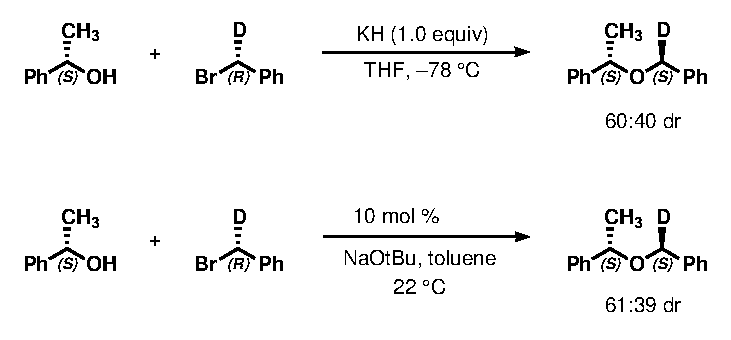
\includegraphics[scale=0.8]{chp_alkylation/images/inversionexpspectra}
  \caption{Data indicates reaction proceeds through an S$_\mathrm{N}$2 mechanism.}
  \label{sch:alkinversionexpspectra}
\end{Scheme}

As a point of comparison, we exposed optically pure (\textit{S})-\ref{cmp:alkaac} to bromide
\ref{cmp:xcao} and potassium hydride in THF at $-$78 \degc\ (\refscheme{alkinversionexpspectra}).
The material recovered was formed in a 60:40 dr based on integration of the $^1$H NMR signals for the benzylic hydrogen attached to the deuterated carbon. Assuming the reaction proceeded through a clean S$_\mathrm{N}$2 mechanism
under these conditions,\footnote{(a) {\frenchspacing Ashby, E. C.; Bae, D. H.; Park, W. S.;
Depriest, R. N.; Su, W. Y. Evidence for Single Electron Transfer in the Reaction of Alkoxides with
Alkyl Halides. \textit{Tetrahedron Lett.} \textbf{1984}, \textit{25}, 5107-5110.} (b)
{\frenchspacing Vollhardt, K. P. C.; Shore, N. E. \textit{Organic Chemistry:
Structure and Function}, 6th ed.; W. H. Freeman and Company: New York, 2011.}} the enantiopurity of bromide
\ref{cmp:xcao} would have been approximately 60:40 er.
We then ran the same experiment under our catalyzed conditions and were surprised to see that the ether was formed
with a nearly identical 61:39 dr, favoring the same diastereomer as the S$_\mathrm{N}$2 control
reaction. These data rule out the possibility of a double inversion mechanism, suggesting that a
pathway other than nucleophilic activation of the electrophile was operative.  



 \subsection{Second Hypothesis: Carbenes as Br\o nsted Bases}
 

 Imidazolium derived carbenes have been described as reasonably strong Br\o nsted
 bases, with p\textit{K}$_\mathrm{a}$ values of the conjugate acids ranging anywhere from 16-24 in
 DMSO.\footnote{{\frenchspacing Alder, R.
 W.; Allen, P.
 R.; Williams, S. J. Stable Carbenes as Strong Bases. \textit{J. Chem. Soc. Chem. Comm.} \textbf{1995},
 1267-1268.}} In 2005, the Movassaghi group reported an NHC catalyzed amidation reaction of
 unactivated esters with amino alcohols.\footnote{{\frenchspacing Movassaghi, M.; Schmidt, M. A.
 \textit{N}-Heterocyclic Carbene-Catalyzed Amidation of Unactivated Esters with Amino Alcohols.
 \textit{Org. Lett.} \textbf{2005}, \textit{7}, 2453-2456.} \label{ref:alkmovcrystal}} In the proposed mechanism, the amino alcohol was primed
 for nucleophilic attack by removing the alcohol proton with the NHC, generating a more
 nucleophilic alkoxide. Careful NMR studies showed that alcohols in the presence of NHCs exhibit a
 significant downfield shift for the \ce{O-H} proton. Movassaghi was also able to obtain a solid
 state structure of IMes complexed with methanol, which showed a nearly linear
 ($\angle$ \ce{C-H-O}, 174$^{\circ}$) hydrogen bond interaction between the methanol and C2 position
 of the imidazolylidene ring (\ref{cmp:alkaau}, \refscheme{alkbronstedbasecycle}). The Scheidt
 group more recently introduced an NHC catalyzed intermolecular \textit{oxa}-Michael
 reaction, where they also propose a Br\o nsted base role for the NHC.\footnote{{\frenchspacing
 Phillips, E.
 M.; Riedrich, M.; Scheidt, K.
 A.
 \textit{N}-Heterocyclic Carbene-Catalyzed Conjugate Additions of Alcohols. \textit{J. Am. Chem.
 Soc.} \textbf{2010}, \textit{132}, 13179-13181.}} In a single intramolecular example, Scheidt
 observed a marginal level of enantioselectivity with a chiral NHC, suggesting that the proton may
 not be fully transferred to the NHC or the imidazolium alkoxide ion-pair was closely associated. 
 
 The proposed catalytic cycle for a Br\o nsted base mechanism, illustrated in
 \refscheme{alkbronstedbasecycle}, again opens with deprotonation of the imidazolium salt
 \ref{cmp:alkaao} to deliver the carbene (\ref{cmp:alkaao}\ce{->i}). The secondary alcohol enters
 the catalytic cycle, forming neutral alcohol carbene complex \textit{ii}. The activated alcohol
 displaces the bromide, forming the ether product and regenerating the imidazolium salt  (\textit{ii}\ce{->}\textit{iii}). The carbene can then be regenerated by deprotonating with an
 additional equivalent of sodium \textit{tert}-butoxide (\textit{iii}\ce{->}\textit{i}).
 
    \begin{Scheme}[t]
 
  \begin{textblock}{1}(10,2)
       \begin{textblock}{1}(-6.5,-1.5) \crossrefcmp{alkaao} \end{textblock}
  \includegraphics[scale=0.3]{chp_alkylation/images/movassaghicrystal}\end{textblock}
  \begin{textblock}{1}(13.5,7.5)
  \includegraphics[scale=0.8]{chp_alkylation/images/movcrystalchemdraw}\end{textblock}
   \begin{textblock}{5}(14,1.4) \small \textsf{\textit{Movassaghi}
  \textbf{2005}\crossref{ref:alkmovcrystal}}\end{textblock}
 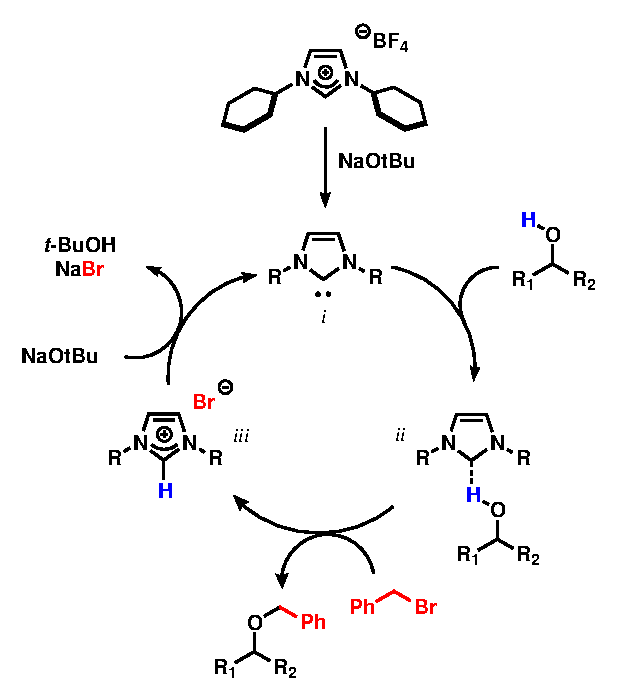
\includegraphics[scale=0.8]{chp_alkylation/images/bronstedbasecycle}
     \begin{textblock}{1}(16.5,-2) \cmp{alkaau} \end{textblock}
  \caption{Proposed cycle for carbene as Br\o nsted base and crystallographic precedents.}
  \label{sch:alkbronstedbasecycle}
\end{Scheme}


 \begin{Scheme}[p]
 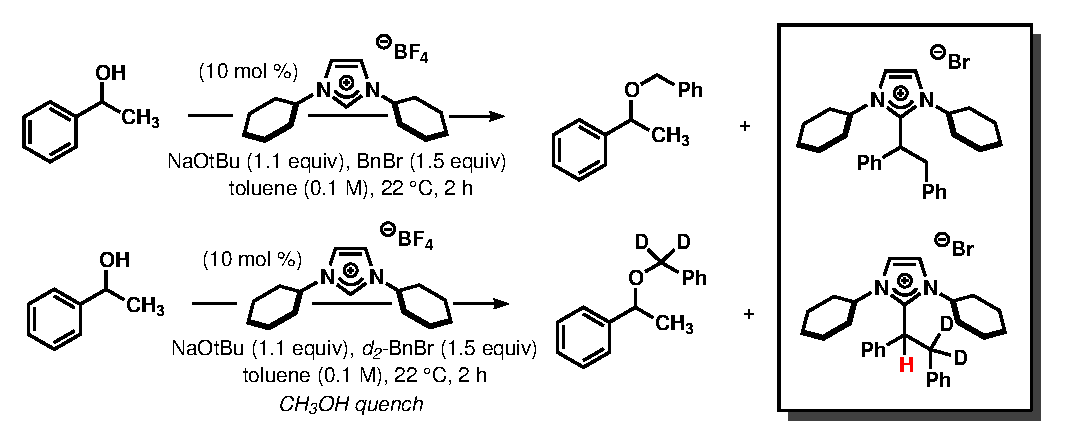
\includegraphics[scale=0.8]{chp_alkylation/images/catalystrecovery}
 \begin{textblock}{1}(5.5,-5.4) \crossrefcmp{alkaao} \end{textblock}
 \begin{textblock}{1}(5.6,-2) \crossrefcmp{alkaao} \end{textblock}
 \begin{textblock}{1}(1.5,-1.4) \crossrefcmp{alkaac} \end{textblock}
 \begin{textblock}{1}(1.5,-4.5) \crossrefcmp{alkaac} \end{textblock}
 \begin{textblock}{1}(10.8,-4.5) \crossrefcmp{xcaa} \end{textblock}
 \begin{textblock}{1}(10.8,-1.4) \crossrefcmp{xcac} \end{textblock}
 \begin{textblock}{1}(14,-6.3) \cmp{xcad} \end{textblock}
 \begin{textblock}{1}(14,-3) \cmp{xcae} \end{textblock}
  \caption{Attempts to recover \ref{cmp:alkaao} lead to the discovery of doubly alkylated salts.}
  \label{sch:alkcatalystrecovery}
\end{Scheme}
   \begin{figure}[p]
   \centering
\vspace{2.1in}
  \begin{textblock}{1}(-1,-9)
  \includegraphics[scale=0.35]{chp_alkylation/images/xray/xcad_nolabels}\end{textblock}
    \begin{textblock}{1}(10,-10)
  \includegraphics[scale=0.45]{chp_alkylation/images/xray/xcai_nolabels}\end{textblock}
 \includegraphics[scale=0.8]{chp_alkylation/images/alkylatedimidazoliums}
 \vspace{10pt}
  \begin{textblock}{1}(2,-3) \crossrefcmp{xcad} \end{textblock}
   \begin{textblock}{1}(12.5,-2) \cmp{xcai} \end{textblock}
  \caption{Crystal structures of C2 alkylated imidazolium salts prepared during this study.}
  \label{fig:alkalkylatedimidazolium}
\end{figure}
 To test this mechanistic hypothesis we were curious if intermediate \textit{iii}, the imidazolium
 salt, could be recovered after the reaction by reprotonating the carbene. The imidazolium
 salt \ref{cmp:alkaao} was virtually insoluble in \ce{Et2O} and fully soluble in \ce{CH2Cl2}, so by
 selective extraction we hoped to cleanly recover the salt.
 At the conclusion of the reaction we concentrated the mixture and removed any organic soluble materials by washing with \ce{Et2O}. The remaining material was dissolved in \ce{CH2Cl2}
 and filtered away from sodium bromide. We were surprised to see that after concentration of the
 \ce{CH2Cl2}, the only salt recovered was doubly alkylated imidazolium \ref{cmp:xcad} in $>$90\%
 purity by $^1$H NMR spectroscopy (\refscheme{alkcatalystrecovery}). The structure of \ref{cmp:xcad}
 was confirmed by careful analysis of the spectral data and ultimately by X-ray crystallography
 (\reffigure{alkalkylatedimidazolium}, left).
 In no situation did we ever recover any of the starting imidazolium salt \ref{cmp:alkaao}.
 When we ran the same experiment with \textit{d}$_2$-benzyl bromide and quenched the reaction with
 methanol, the recovered salt contained only two deuteriums (\ref{cmp:xcae}). A proton was
 incorporated at the benzylic methine carbon, indicating that it was deprotonated at some point
 during the reaction.
 These data seemed to support a mechanism comparable to the original proposal based on a
 nucleophilic activation role for the carbene (\refscheme{alkactivationcycleone}, page
 \pageref{sch:alkactivationcycleone}).
 


We were able to independently synthesize an authentic sample of the doubly alkylated imidazolium
salt
\ref{cmp:xcad} in high yield by adding excess sodium \textit{tert}-butoxide and benzyl bromide to a
THF solution of \ref{cmp:alkaao}. With sufficient quantities of material in hand, we carried out a
series of experiments to try to understand the role of the alkylated imidazolium
(\refscheme{alkdibenzylcontrols}). In the absence of benzyl bromide and with stoichiometric
\ref{cmp:xcad} none of the desired product was detectable, consistent with the previous experiment which showed the
reaction proceeds through an S$_\mathrm{N}$2 pathway (\refscheme{alkinversionexpspectra}, page
\pageref{sch:alkinversionexpspectra}). Transfer of a benzyl group from \ref{cmp:xcad} would require
a double inversion of the electrophile which was formerly ruled out. With a catalytic amount of
\ref{cmp:xcad} and 1.5 equivalents of benzyl bromide the yield increased to 70\%, a result
suspiciously similar to the yield obtained with the parent imidazolium salt \ref{cmp:alkaao} (74\%). 
 \begin{Scheme}[b]
 \centering
 \includegraphics[scale=0.8]{chp_alkylation/images/dibenzylcontrols}
  \begin{textblock}{1}(7.5,-2.8) \crossrefcmp{xcad} \end{textblock}
  \begin{textblock}{1}(14.4,-2.3) \crossrefcmp{xcad} \end{textblock}
  \begin{textblock}{1}(1.5,-1) \crossrefcmp{alkaac} \end{textblock}
  \begin{textblock}{1}(11.2,-1) \crossrefcmp{xcaa} \end{textblock}
   \begin{textblock}{1}(17.95,-2.3) \crossrefcmp{xcaa} \end{textblock}
    \caption{Experiments with C2 alkylated imidazolium salt \ref{cmp:xcad}.}
  \label{sch:alkdibenzylcontrols}
\end{Scheme}

Given that we recovered \ref{cmp:xcae} (\refscheme{alkcatalystrecovery}) with a proton incorporated
at the benzylic methine position, this data point seemed to suggest a role for an anion adjacent to
the imidazolium ring. We attempted to prepare a catalyst with a quaternary carbon attached to the C2
position of the imidazolium to remove any hydrogens. Exposure of \ref{cmp:alkaao} to 5 equivalents
of methyl iodide and 4 equivalents of potassium \textit{tert}-butoxide did not deliver the
anticipated quaternary substituted imidazolium salt even with prolonged heating and sonication of
the heterogeneous mixture (\ce{->}\ref{cmp:alkaav}, \refscheme{alkisopropylimidazoliumprep}).
Instead, a 69\% isolated yield of the isopropyl substituted salt \ref{cmp:xcag} was obtained. A
solid state structure of the tetraphenyl borate salt (\ref{cmp:xcai}, \reffigure{alkalkylatedimidazolium})
showed that significant amount of allylic strain would be generated upon introduction of the
\textit{tert}-butyl group, likely explaining why the reaction failed to introduce an
additional methyl group.\footnote{The \ce{C16-C1-N2-C10} dihedral angle was 5.2$^{\circ}$ in the
solid state structure.
See the appendix for further details.} Carrying out the reaction with a catalytic amount of
isopropyl substituted imidazolium iodide salt \ref{cmp:xcag} delivered the ether product in 82\%
yield, the highest yield observed up to this point. While this data point does not rule out the possible involvement of the proton adjacent to
the imidazolium ring, it does point to a mechanistic pathway that does not require the involvement
of a C2 carbene.
 \begin{Scheme}[t]
 \centering
 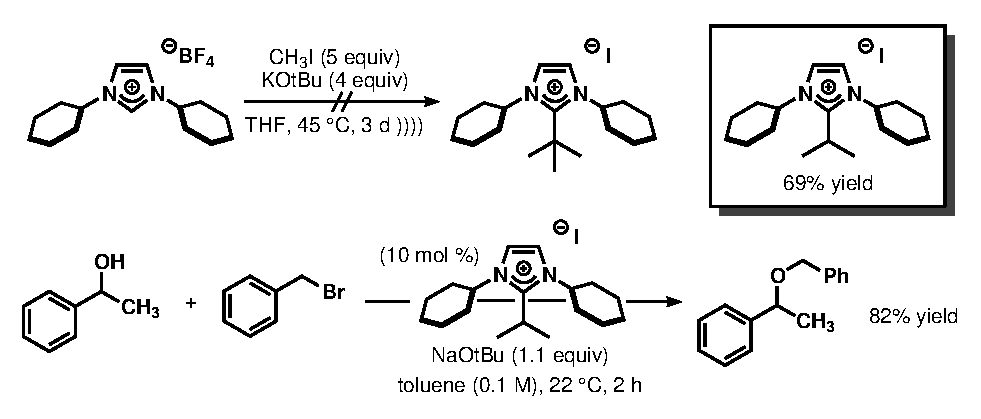
\includegraphics[scale=0.8]{chp_alkylation/images/isopropylimidazoliumprep}
\begin{textblock}{1}(3.2,-4.5) \crossrefcmp{alkaao} \end{textblock}
\begin{textblock}{1}(2.6,-0.8) \crossrefcmp{alkaac} \end{textblock}
\begin{textblock}{1}(15,-0.8) \crossrefcmp{xcaa} \end{textblock}
\begin{textblock}{1}(9.4,-6) \cmp{alkaav} \end{textblock}
\begin{textblock}{1}(14.3,-6) \cmp{xcag} \end{textblock}
\begin{textblock}{1}(12,-2.5) \crossrefcmp{xcag} \end{textblock}
    \caption{Attempted substitution of C2 position with quaternary carbon.}
  \label{sch:alkisopropylimidazoliumprep}
\end{Scheme}


 \subsection{Loosely Associated Ion-Pair Mechanism}
 The experiments in the previous two sections showed that an intermediate involving
a carbene in the catalytic cycle was highly unlikely. Alkylation of the imidazolium ring at the C2
position effectively blocks the formation of a carbene,\footnote{Abnormal carbenes at the C4 or C5
positions of imidazoliums have been reported but we did not believe this was a likely
intermediate.
{\frenchspacing Arnold, P.
L.; Pearson, S.
Abnormal
\textit{N}-Heterocyclic Carbenes. \textit{Coordin. Chem. Rev.} \textbf{2007}, \textit{251}, 596-609.}} yet the salts were still competent
catalysts. We were still curious if there was a role for the benzylic methine proton adjacent to the
imidazolium ring. A study of base loading versus yield of \ref{cmp:alkaac} revealed a linear
increase (R$^2$ = 0.99) in yield up to 1.3 equivalents of base, and a significant drop in yield
beyond 1.4 equivalents (\reffigure{alkbaseloadingstudy}). The reaction was highly sensitive even to
subtle changes in the amount of base, suggesting a proton transfer event may be critical in the
reaction mechanism. 
\begin{figure}[h]
  \centering
  \includegraphics[scale=0.55, trim = 15mm 45mm 15mm 30mm,
clip]{chp_alkylation/images/baseloadingscreen}
\vspace{5pt}
  \caption{Base loading study, equivalents of NaOtBu versus product yield.}
  \begin{textblock}{3}(-1,-8)  \begin{sideways}\footnotesize
  \textbf{\textsf{Yield \ref{cmp:alkaac} (\%)}} \end{sideways}
  \end{textblock}
\begin{textblock}{5}(7,-1.2)  \footnotesize \textbf{\textsf{Equivalents NaOtBu}}
\end{textblock}
\begin{textblock}{10}(1,-11)  \footnotesize \textsf{\textit{Conditions:}\\ 10 mol \%
\ref{cmp:alkaao}, 1.5 equiv BnBr \\ toluene (0.1 M), 22 \degc, 2 h }
\end{textblock}
 \label{fig:alkbaseloadingstudy}
\end{figure}

 \begin{Scheme}[t]
 \centering
 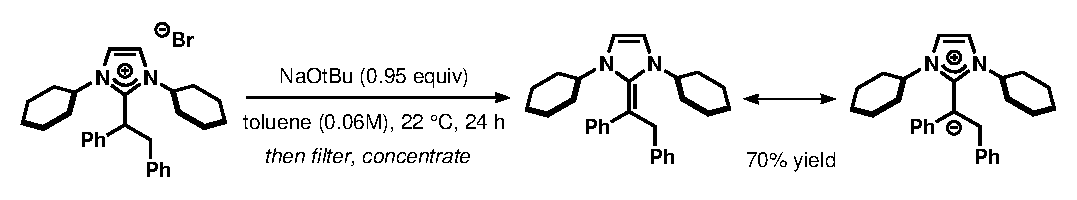
\includegraphics[scale=0.8]{chp_alkylation/images/ylidepreparation}
\begin{textblock}{1}(0.7,-2.6) \crossrefcmp{xcad} \end{textblock}
\begin{textblock}{1}(9.8,-2.6) \cmp{xcal} \end{textblock}
    \caption{Deprotonation of imidazolium salt \ref{cmp:xcad} to afford ylide \ref{cmp:xcal}. }
  \label{sch:alkylidepreparation}
\end{Scheme}
We were able to cleanly deprotonate dibenzylated imidazolium bromide salt \ref{cmp:xcad} with sodium
\textit{tert}-butoxide in toluene, conditions comparable to our standard reaction conditions
(\refscheme{alkylidepreparation}).
After filtration inside an inert atmosphere glove box to remove any residual \ref{cmp:xcad} and
sodium bromide, concentration afforded a pure dark green solid in 70\% yield
(\ce{->}\ref{cmp:xcal}).
Dilute toluene or benzene solutions of \ref{cmp:xcal} were bright yellow, consistent with some of the earlier color changes observed in the
reaction (\refscheme{alkactivationcycleone}, page \pageref{sch:alkactivationcycleone}). The $^1$H
and $^{13}$C NMR data for \ref{cmp:xcal} showed considerable \textit{C}$_s$ symmetry, indicative of
significant ylide or single bond character. The symmetry could be the result of free rotation, or an orthogonal
relationship between the phenyl groups and the imidazole ring. 

\begin{Scheme}[h]
 \centering
 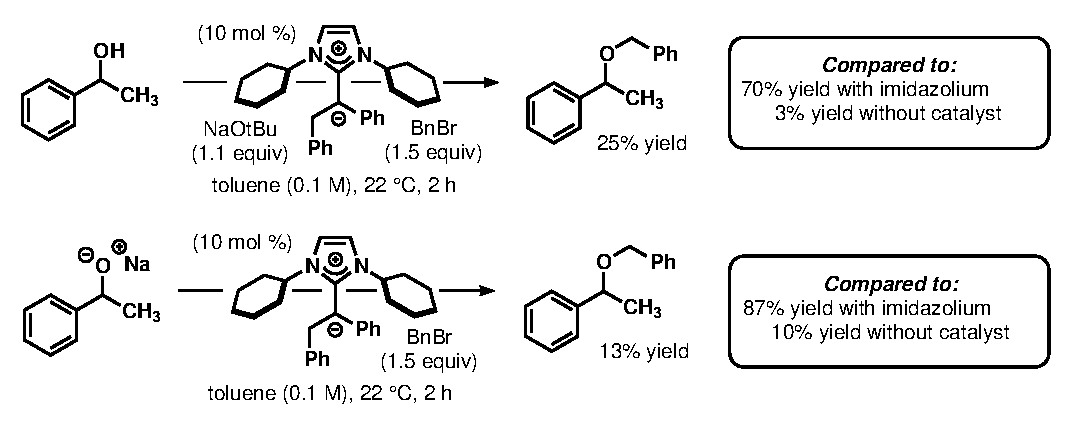
\includegraphics[scale=0.8]{chp_alkylation/images/ylidecontrols}
\begin{textblock}{1}(1.7,-4.5) \crossrefcmp{alkaac} \end{textblock}
\begin{textblock}{1}(11,-4.3) \crossrefcmp{xcaa} \end{textblock}
\begin{textblock}{1}(11,-0.6) \crossrefcmp{xcaa} \end{textblock}
  \begin{textblock}{1}(1.8,-0.6) \crossrefcmp{alkaap} \end{textblock}
  \begin{textblock}{1}(7.5,-3) \crossrefcmp{xcal} \end{textblock}
   \begin{textblock}{1}(7.5,-6.8) \crossrefcmp{xcal} \end{textblock}
   \begin{textblock}{1}(18.1,-1.95) \crossrefcmp{xcad} \end{textblock}
  \begin{textblock}{1}(18.1,-5.83) \crossrefcmp{xcad} \end{textblock}
    \caption{Experiments with ylide \ref{cmp:xcal} showed poorer yields than the parent imidazolium
    salt \ref{cmp:xcad}.}
  \label{sch:alkylidecontrols}
\end{Scheme}
\begin{Scheme}[t]
 \centering
 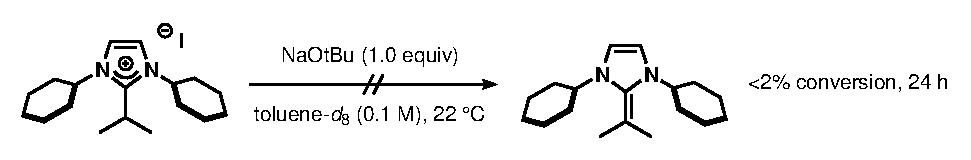
\includegraphics[scale=0.8]{chp_alkylation/images/isopropylylide}
\begin{textblock}{1}(1.8,-1.8) \crossrefcmp{xcag} \end{textblock}
 \begin{textblock}{1}(10.5,-1.8) \cmp{alkaaw} \end{textblock}
%   \begin{textblock}{1}(7.3,-2.8) \crossrefcmp{xcad} \end{textblock}
%   \begin{textblock}{1}(14,-2.3) \crossrefcmp{xcad} \end{textblock}
%   \begin{textblock}{1}(1.1,-1) \crossrefcmp{alkaac} \end{textblock}
%   \begin{textblock}{1}(11,-1) \crossrefcmp{xcaa} \end{textblock}
%    \begin{textblock}{1}(17.65,-2.3) \crossrefcmp{xcaa} \end{textblock}
    \caption{Attempts to form ylide from \ref{cmp:xcag} were unsuccessful.}
  \label{sch:alkisopropylylide}
\end{Scheme}

To test the catalytic activity of \ref{cmp:xcal}, we subjected it to two different experiments.
Under standard conditions with 1-phenylethanol, a substantially lower 25\% yield of ether
\ref{cmp:xcaa} was observed (\refscheme{alkylidecontrols}, top). In contrast, the protonated
imidazolium salt \ref{cmp:xcad} gave a 70\% yield in the same time frame under identical conditions. The 25\% yield was still higher than the uncatalyzed background
reaction, suggesting that ylide \ref{cmp:xcal} could be a resting state of the more active
imidazolium catalyst that can slowly re-enter the catalytic cycle upon protonation. The base loading study was also
consistent with this observation. Higher loadings of base lead to a decrease in yield, presumably by
funnelling more of the catalyst to the less active deprotonated form. Starting with the sodium
alkoxide of 1-phenylethanol delivered the product in a marginal 13\% yield, within experimental error of the
uncatalyzed background reaction. The same reaction with imidazolium salt \ref{cmp:xcad} afforded a
significantly augmented 87\% yield.  When we attempted to form the analogous ylide with \ref{cmp:xcag}, $<$2\%
conversion occured in 24 hours by $^1$H NMR (\ce{->}\ref{cmp:alkaaw}, \refscheme{alkisopropylylide}). The
slightly higher yield obtained with \ref{cmp:xcag} (82\% versus 70\% with \ref{cmp:xcad}) could be
attributed to the fact that the isopropyl group methine proton was significantly less acidic and
production of the deactivated form of the catalyst was not as facile. 

\begin{Scheme}[h]
 \centering
 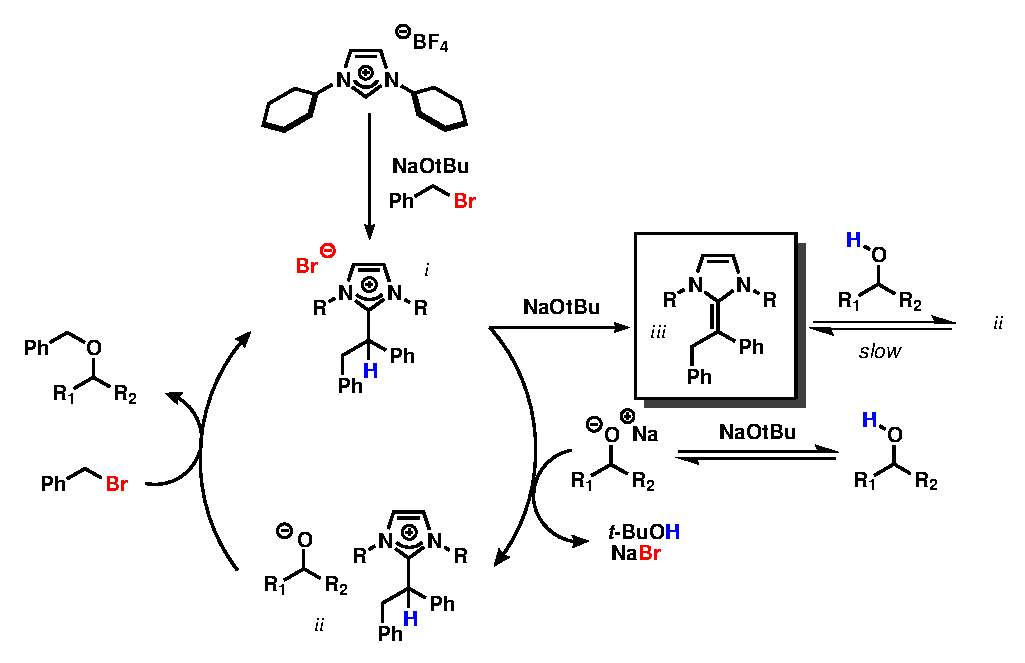
\includegraphics[scale=0.8]{chp_alkylation/images/counterionmechbenzyl}
 \begin{textblock}{1}(5.5,-10.7) \crossrefcmp{alkaao} \end{textblock}
    \caption{Proposed mechanism consistent with all of the data points.}
  \label{sch:alkcounterionmechbenzyl}
\end{Scheme}


The experimental evidence points to the mechanistic proposal illustrated in
\refscheme{alkcounterionmechbenzyl}. Before entering the catalytic cycle, \ref{cmp:alkaao} rapidly
undergoes double benzylation to produce the active catalyst (\ref{cmp:alkaao}\ce{->}\textit{i}). The sodium alkoxide of the secondary alcohol, in
equilibrium with sodium \textit{tert}-butoxide, exchanges for the bromide counter-ion causing sodium
bromide to precipitate from the reaction mixture (\textit{i}\ce{->}\textit{ii}). The alkoxide, now
paired with a weakly associated and diffuse counter-ion, displaces benzyl bromide to deliver the
product and regenerate the catalyst (\textit{ii}\ce{->}\textit{i}). Alternatively, the catalyst can be
deprotonated by sodium \textit{tert}-butoxide to generate the inactive ylide form
(\textit{i}\ce{->}\textit{iii}). The ylide can slowly re-enter the catalytic cycle upon protonation
from the secondary alcohol (\textit{iii}\ce{->}\textit{ii}).

During the course of our studies, we had also prepared a series of catalysts with different
counter-ions and were initially perplexed by the results (\refscheme{alkweakcounterions}). Catalysts with larger and more weakly coordinating
ions lead to diminishing yields of \ref{cmp:xcaa}. Our hope was that by increasing the solubility of
the catalyst, we should see a corresponding increase in the yield. The critical step in the proposed
mechanism requires the formation of an imidazolium alkoxide ion-pair (\textit{i}\ce{->}\textit{ii}). The formation of the integral ion-pair could be driven by the precipitation of sodium bromide, and with
other more soluble counter-ions this key exchange may not occur as
readily.\footnote{For a discussion on solubility of weakly coordinated ions in low
dielectric media see: {\frenchspacing Krossing, I.; Raabe, I.
Noncoordinating Anions--Fact or Fiction? A Survey of Likely Candidates.
\textit{Angew. Chem. Int. Ed.} \textbf{2004}, \textit{43}, 2066-2090.}} These observations are
consistent with the proposed mechanistic pathway in \refscheme{alkcounterionmechbenzyl}.

\begin{Scheme}[h]
 \centering
 \includegraphics[scale=0.8]{chp_alkylation/images/weakcounterions}
 \begin{textblock}{1}(1.6,-0.8) \crossrefcmp{alkaac} \end{textblock}
  \begin{textblock}{1}(10.7,-0.8) \crossrefcmp{xcaa} \end{textblock}
   \begin{textblock}{1}(13.5,-2.7) \crossrefcmp{xcag} \end{textblock}
   \begin{textblock}{1}(13.5,-2.15) \cmp{xcah} \end{textblock}
   \begin{textblock}{1}(13.5,-1.65) \crossrefcmp{xcai} \end{textblock}
   \begin{textblock}{1}(13.5,-1.15) \cmp{xcaj} \end{textblock}
    \caption{Diminishing yields with larger and less coordinating anions.}
  \label{sch:alkweakcounterions}
\end{Scheme}

\pagebreak
\section{Transition State Structure Experiments}

Previous screening had shown that commercially available aryl-substituted imidazolium salts
containing \textit{ortho} substitution were not competent catalysts
(\refscheme{alkimidazoliumscreen}, page \pageref{sch:alkimidazoliumscreen}). Given the new
information about the mechanism, it was plausible that these catalysts were inactive because they
could not form the active doubly-alkylated catalyst \textit{in situ}. 
\begin{figure}[h]
 \centering
 \begin{textblock}{1}(7.5,-0.8)  \includegraphics[scale=0.55]{chp_alkylation/images/xcag_lumo}
 \end{textblock}
   \begin{textblock}{1}(-1,-0.8) 
  \includegraphics[scale=0.33]{chp_alkylation/images/xray/xcaf_frontview} \end{textblock} 
     \begin{textblock}{1}(3.5,7.5) 
  \includegraphics[scale=0.8]{chp_alkylation/images/xcaf_nobox} \end{textblock} 
       \begin{textblock}{1}(13.5,8) 
  \includegraphics[scale=0.8]{chp_alkylation/images/xcag_nobox_noi} \end{textblock} 
     \begin{textblock}{1}(3.4,8) \cmp{xcaf} \end{textblock} 
\vspace{3.3in}
  \caption{Crystal structure of \ref{cmp:xcaf} (left) and imidazolium LUMO (right) --
    \textit{Gaussian '03 - AM1}}
  \label{fig:alkmescrystalandlumo}
\end{figure}
We prepared an authentic sample of doubly-benzylated IMes (\ref{cmp:xcaf},
\reffigure{alkmescrystalandlumo}, left) and found that even with pre-alkylation, the catalyst was
not active. However, the solid state structure of \ref{cmp:xcaf} led to a hypothesis about the method of
interaction between the imidazolium and alkoxide. Low level computation modeling of the imidazolium
LUMO  showed a large coefficient centered on the C2 position between
the two nitrogens (\reffigure{alkmescrystalandlumo}, right). It was possible that the \textit{ortho}
substitution on the aryl groups blocked access to the LUMO, weakening the interaction between the catalyst and alkoxide.\footnote{Attempts to
prepared other unhindered and electronically modified aryl-imidazolium salts (aryl = phenyl,
\textit{p}-\ce{OCH3} phenyl, \textit{p}-\ce{NO2} phenyl) were unsuccessful.} While this would
generate a less nucleophilic alkoxide, we hypothesized that the formation of a neutral C2 adduct
could be a solubilizing interaction in the low dielectric solvent. \begin{Scheme}[t]
 \centering
 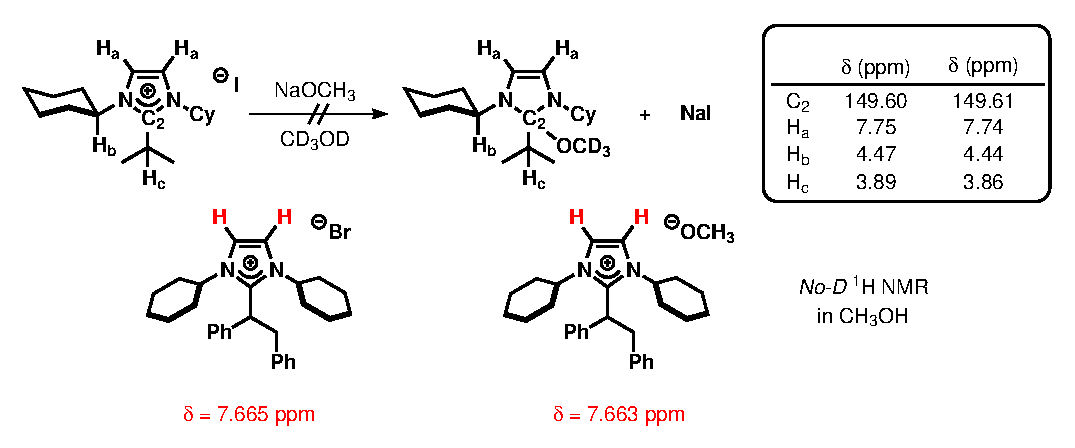
\includegraphics[scale=0.8]{chp_alkylation/images/lumoadditionnmr}
  \begin{textblock}{1}(0.8,-7) \crossrefcmp{xcag} \end{textblock}
  \begin{textblock}{1}(7.7,-7) \cmp{alkaax} \end{textblock}
  \begin{textblock}{1}(2.5,-3.5) \crossrefcmp{xcad} \end{textblock}
  \begin{textblock}{1}(8.7,-3.5) \cmp{alkaay} \end{textblock}
   \begin{textblock}{1}(15.5,-7.05) \crossrefcmp{xcag} \end{textblock}
\begin{textblock}{1}(17.4,-7.05) \crossrefcmp{alkaax} \end{textblock}
%    \begin{textblock}{1}(13.5,-2.7) \crossrefcmp{xcag} \end{textblock}
%    \begin{textblock}{1}(13.5,-2.15) \cmp{xcah} \end{textblock}
%    \begin{textblock}{1}(13.5,-1.65) \crossrefcmp{xcai} \end{textblock}
%    \begin{textblock}{1}(13.5,-1.15) \cmp{xcaj} \end{textblock}
     \caption{NMR data indicates alkoxide not bound to C2 position.}
  \label{sch:alklumoadditionnmr}
\end{Scheme}

A covalent interaction between the alkoxide and imidazolium was tested by a series of NMR
experiments (\refscheme{alklumoadditionnmr}). Covalent interaction between the imidazolium C2 and
alkoxide would dearomatize the ring and lead to significant differences in the chemical
shifts relative to the halide salts.  Treatment of imidazolium iodide \ref{cmp:xcag} with
freshly prepared \ce{NaOCH3} showed effectively no change in the proton and carbon NMR chemical
shifts (\ce{->}\ref{cmp:alkaax}). Furthermore, proton NMR data for \ref{cmp:xcad} and the
corresponding methoxide salt \ref{cmp:alkaay}\footnote{Prepared by adding methanol to ylide
\ref{cmp:xcal}.
See the experimental section for characterization data.} exhibited identical proton shifts in methanol for the C4 and C5 hydrogens.
These experiments do not completely rule out the possibility of a fleeting covalent interaction in a highly unfavorable equilibrium with the
dissociated form. For solubility reasons, methanol was used as the solvent for these experiments.
The use of methanol could discourage formation of the neutral dearomatized adduct \ref{cmp:alkaax} by
stabilizing the charge separated form. This appears to be the case with \ref{cmp:xcad} and
\ref{cmp:alkaax}, as there is essentially no difference in the proton spectra even with the
different counterions. 

In an attempt to understand how intimately associated the imidazolium alkoxide ion-pair was, a
\textit{C}$_2$-symmetric chiral catalyst (\ref{cmp:xcak}) was prepared to look for any kinetic
resolution of the secondary alcohol (\reftable{alkchiralcat}). We were pleased to see with 1.3
equivalents of sodium \textit{tert}-butoxide the reaction rapidly reached complete conversion
(entry 1). Dropping the base loading to 0.75 equivalents delivered the product in 55\% yield,
consistent with 0.2 equivalents of base consumed during the formation of the doubly-alkylated active
catalyst. Unfortunately both the product (\ref{cmp:xcaa}) and starting material (\ref{cmp:alkaac})
were racemic (entry 2). Carrying out the reaction at lower temperatures also did not
afford material in any detectable levels of enantioselectivity (entries 3 and 4). These data suggest
that  the ions were weakly associated in a manner that was poorly organized.\footnote{Several other
secondary alcohols were tested and all in all cases racemic starting materials and products
were recovered.}

\singlespacing
\ctable[
	caption = Chiral \textit{C}$_2$-symmetric catalyst \ref{cmp:xcak} shows no asymmetric induction.,
	label = nowidth,
	pos = t,
	label = tbl:alkchiralcat,
	doinside = \footnotesize,
	botcap,
	notespar
]{ccccccc}{
	\tnote{\textit{Conditions:} 0.1 M in toluene with 10 mol \% \ref{cmp:xcak}, 1.5 equiv
	benzyl bromide. Catalyst \ref{cmp:xcak} and NaOtBu pre-mixed for 15 minutes at 22 \degc\  before
	adding benzyl bromide and cooling to the appropriate temperature.}
	\tnote[b]{Determined by chiral GC analysis in comparison with authentic racemic material.}
	\tnote[c]{Determined by $^1$H NMR with 1,3,5-trimethoxybenzene as an internal standard.}

 	\begin{textblock}{1}(6.3,-8.4) \cmp{xcak} \end{textblock}
 	\begin{textblock}{1}(1.5,-6.5) \crossrefcmp{alkaac} \end{textblock}
 	\begin{textblock}{1}(14,-6.5) \crossrefcmp{xcaa} \end{textblock}
}{
\multicolumn{7}{c}{
\includegraphics[scale=0.8]{chp_alkylation/images/chiralcathead} 
} \\
\FL
%%% begin header line
 entry\tmark & equiv base  &  temp (\degc) & er \ref{cmp:alkaac}\tmark[b] &  er
 \ref{cmp:xcaa}\tmark[b] & k$_\mathrm{rel}$ &  yield \ref{cmp:xcaa} (\%)\tmark[c]  \ML 
%% end header line, begin data
1 & 1.3 & 22 & \textit{na} & \textit{na} & \textit{na} & $>$98  \\
\rowcolor{gray!15}2 & 0.75 & 22 & 50:50 & 50:50 & 1 & 55 \\
3 & 0.75 & 0 & 52:48 & 51:49 & 1.06 & 46 \\
4 & 0.75 & $-$78 & 50:50 & 50:50 & 1 & 9\LL}
\doublespacing

\vspace{-11pt}
Computations on imidazolium methoxide geometries in toluene solution lead to another plausible
hypothesis for the how the two ions interact in solution. Geometry optimization calculations seemed
to suggest that there was a considerable degree of hydrogen bonding between the C4 imidazolium
hydrogen and the alkoxide (\reffigure{alkimidazoliumalkoxidecalc}).  The C4--H bond length of
1.20 \AA\  was signifcantly elongated relative to the C5--H bond length of just 1.08 \AA. The solid
state structures of \ref{cmp:xcad} (page \pageref{cmp:xcad}) and \ref{cmp:xcaf} (page
\pageref{cmp:xcaf}) also seemed to show the halide counter-ion associated with a single C4 hydrogen.\footnote{Carbon hydrogen bond lengths were not accurately determined in the solid state
structures. The orientation of the halide relative to the imidazolium ring may have simply been the
result of a preferred crystal packing orientation. See the appendix for details.} Reexamining the
data for the catalysts illustrated in \reffigure{alkimidazoliumalkoxidecalc} showed a clear trend.
The most successful catalysts were those with unsaturated \textit{sp}$^2$ hybridized backbones
containing two hydrogens. When we recorded NMR data for ylide \ref{cmp:xcal} in deuterated methanol
we expected to see deuterium incorporated at the benzylic methine position, but we were surprised to
see that the signals associated with the C4 and C5 positions also exchanged
(\ce{->}\ref{cmp:xcam}, \refscheme{alkdeuteriumexchange}, top).
\begin{figure}[t]
\vspace{2.5in}
   \begin{textblock}{1}(-3,-9.5)
   \includegraphics[scale=0.37]{chp_alkylation/images/imidazolium_methoxide}
   \end{textblock}
   \begin{textblock}{1}(1.2,-8.3)\includegraphics[scale=0.8]{chp_alkylation/images/imidazolium_methoxide_overlay}
   \end{textblock}
      \begin{textblock}{1}(10,-9)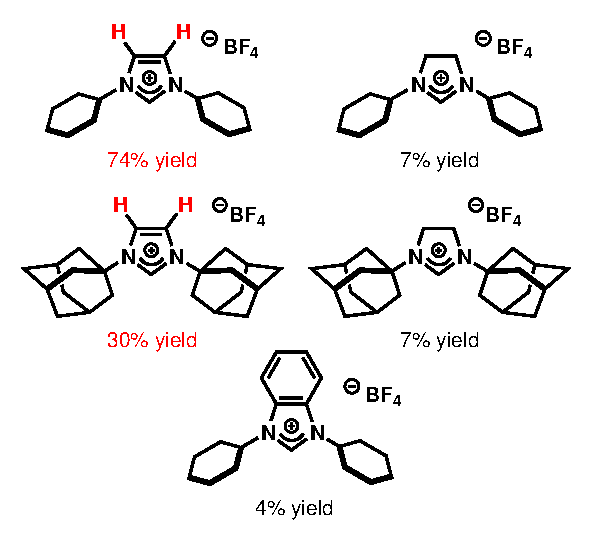
\includegraphics[scale=0.8]{chp_alkylation/images/backbonehydrogencats}
   \end{textblock}
   \vspace{15pt}
     \caption{Computations suggest role for C4 and C5 protons -- \textit{Gaussian '03 -
     B3LYP/6-31G*}}
  \label{fig:alkimidazoliumalkoxidecalc}
\end{figure}
\begin{Scheme}[b]
 \centering
 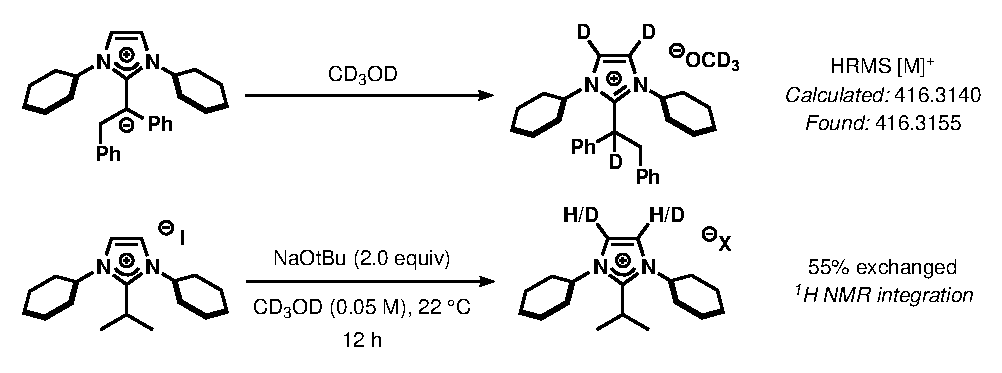
\includegraphics[scale=0.8]{chp_alkylation/images/deuteriumexchange}
 \begin{textblock}{1}(1.3,-5.9)\crossrefcmp{xcal}\end{textblock}
  \begin{textblock}{1}(1.3,-2.1)\crossrefcmp{xcag}\end{textblock}
  \begin{textblock}{1}(10,-5.7)\cmp{xcam}\end{textblock}
  \begin{textblock}{1}(10,-2.1)\cmp{alkaaz}\end{textblock}
     \caption{Protons at C4 and C5 positions are exchangable under basic conditions.}
  \label{sch:alkdeuteriumexchange}
\end{Scheme}
Exposure of imidazolium \ref{cmp:xcag} to sodium \textit{tert}-butoxide in deuterated methanol
showed a slow 55\% exchange of \textit{only} the backbone hydrogens in 12 hours
(\ce{->}\ref{cmp:alkaaz}, \refscheme{alkdeuteriumexchange}, bottom). Weak \ce{C-H\bond{...}O}
hydrogen bonds are known to exist and given the propensity for these hydrogens to exchange under basic conditions, we
believed this might be a plausible secondary interaction between the catalyst and alkoxide.\footnote{{\frenchspacing Taylor, R.; Kennard, O.
Crystallographic Evidence for the Existence of \ce{C-H\bond{...}O}, \ce{C-H\bond{...}N} and \ce{C-H\bond{...}Cl} Hydrogen Bonds.
\textit{J. Am. Chem. Soc.} \textbf{1982}, \textit{104}, 5063-5070.}}


While there was good evidence that the hydrogens may be important, we needed to prepare an
imidazolium salt with alkyl substitution at the C4 and C5 positions. Synthesizing a
penta-substituted imidazolium proved to be a significant challenge, but through the use of microwave chemistry we were
able to access 4,5-dimethyl imidazolium \ref{cmp:xcanb}
(\refscheme{alkdibenzylscreen}).\footnote{{\frenchspacing Wolkenberg, S. E.; Wisnoski, D. D.;
Leister, W. H.; Wang, Y.; Zhao, Z.; Lindsley, C. W. Efficient Synthesis of Imidazoles from Aldehydes and 1,2-Diketones Using Microwave Irradiation. \textit{Org. Lett.} \textbf{2004}, \textit{6}, 1453-1456.}} The results in \refscheme{alkdibenzylscreen} clearly show that there was no difference in chemical yield after two hours with methyl substitution or hydrogens on the C4 and C5 positions. These data points
confirm that the backbone hydrogens were not an integral catalyst feature and suggest that the
alkoxide interaction was predominantly ionic in nature.\footnote{{\frenchspacing Macchioni, A. Ion
Pairing in Transition-Metal Organometallic Chemistry. \textit{Chem. Rev.} \textbf{2005},
\textit{105}, 2039-2073.}} 
 \begin{Scheme}[h]
 \centering
 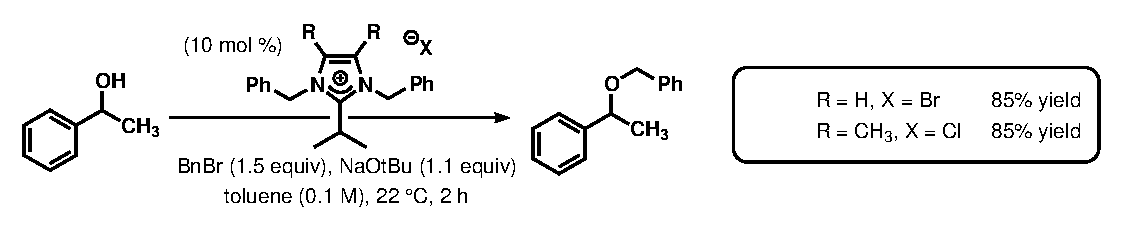
\includegraphics[scale=0.8]{chp_alkylation/images/dibenzylscreen}
   \begin{textblock}{1}(13.3,-2.15)\cmp{xcan}\end{textblock}
   \begin{textblock}{1}(13.3,-1.6)\cmp{xcanb}\end{textblock}
     \caption{Protons at C4 and C5 position not required for catalytic activity.}
  \label{sch:alkdibenzylscreen}
\end{Scheme}

\pagebreak
 \section{Conclusions}
 Numerous examples of stereoselective reactions catalyzed
by chiral ion-pairs have been reported in the literature. Strategies based on
phase-transfer catalysis are among the most common and well studied.\footnote{For pioneering reports
see:
(a) {\frenchspacing Dolling, U. H.; Davis, P.; Grabowski, E. J. J. Efficient Catalytic Asymmetric
Alkylations. 1. Enantioselective Synthesis of (+)-Indacrinone \textit{via} Chiral Phase-Transfer
Catalysis. \textit{J. Am. Chem. Soc.} \textbf{1984}, \textit{106}, 446-447.} (b) {\frenchspacing
Corey, E. J.; Xu, F.; Noe, M. C. A Rational Approach to Catalytic Enantioselective Enolate
Alkylation Using a Structurally Rigidified and Defined Chiral Quaternary Ammonium Salt Under Phase
Transfer Conditions. \textit{J. Am. Chem. Soc.} \textbf{1997}, \textit{119}, 12414-12415.} (c)
{\frenchspacing Ooi, T.; Kameda, M.; Maruoka, K. Molecular Design of a \textit{C}$_2$-Symmetric
Chiral Phase-Transfer Catalyst for Practical Asymmetric Synthesis of $\alpha$-Amino Acids.
\textit{J. Am. Chem. Soc.} \textbf{1999}, \textit{121}, 6519-6520.} For reviews see: (d)
{\frenchspacing O�Donnell, M. J. The Enantioselective Synthesis of $\alpha$-Amino Acids by
Phase-Transfer Catalysis with Achiral Schiff Base Esters. \textit{Acc. Chem. Res.} \textbf{2004},
\textit{37}, 506-517.} (e) {\frenchspacing Ooi, T.; Maruoka, K. Recent Advances in Asymmetric
Phase-Transfer Catalysis. \textit{Angew. Chem. Int. Ed.} \textbf{2007}, \textit{46}, 4222-4266.}}
Chiral crown ethers have also been used under single-liquid phase conditions to sequester potassium ions while remaining closely associated with the substrate to impart stereoselectivity.\footnote{(a) {\frenchspacing Cram, D.
J.; Sogah, G.
D.
Y.
Chiral Crown Complexes Catalyse Michael Addition Reactions to Give Adducts in High Optical Yields. \textit{J. Chem. Soc.
Chem. Comm.} \textbf{1981}, 625-628.} (b) {\frenchspacing Aoki, S.; Sasaki, S.; Koga, K. Simple
Chiral Crown Ethers Complexed with Potassium \textit{tert}-Butoxide as Efficient Catalysts for
Asymmetric Michael Additions. \textit{Tetrahedron Lett.} \textbf{1989}, \textit{30}, 7229-7230.}}
More recently the Jacobsen group and others have utilized chiral thioureas as ``anion-binding''
catalysts to generate chiral ion pairs with cationic substrates.\footnote{For lead references see:
(a) {\frenchspacing Raheem, I. T.; Thiara, P. S.; Peterson, E. A.; Jacobsen, E. N. Enantioselective
Pictet-Spengler-Type Cyclizations of Hydroxylactams: H-Bond Donor Catalysis by Anion Binding.
\textit{J. Am. Chem. Soc.} \textbf{2007}, \textit{129}, 13404-13405.} (b) {\frenchspacing Zuend, S. J.; Jacobsen, E. N. Mechanism of Amido-Thiourea Catalyzed Enantioselective Imine Hydrocyanation: Transition State Stabilization \textit{via} Multiple Non-Covalent Interaction. \textit{J. Am. Chem. Soc.} \textbf{2009}, \textit{131}, 15358-15374.} (c)
{\frenchspacing Knowles, R. R.; Jacobsen, E. N. Attractive Noncovalent Interactions in Asymmetric
Catalysis: Links Between Enzymes and Small Molecule Catalysts. \textit{Proc. Natl. Acad. Sci. USA}
\textbf{2010}, \textit{107}, 20678-20685.}}
Future chiral catalyst designs, based on these mechanistic studies the aforementioned reports from
the literature, will likely need to incorporate more functional groups that can engange in
well-defined non-covalent secondary interactions (H-bonding, cation-$\pi$, $\pi$-$\pi$, etc\ldots) to create more organized
transition states.

In summary, we have laid the groundwork for a new class of cationic organocatalysts that are capable
of constructing \ce{C-O} bonds. Careful mechanistic studies first ruled out the possible
involvment of carbenes and lead to the discovery of unusual C2 alkylated imidazolium
salts.\crossref{ref:alkwangelin} Further mechanistic experiments showed that the reaction can be
catalyzed by penta-substituted imidazolium salts, suggesting the catalyst interacts in largely ionic
fashion with the substrate. While catalytic Williamson ether reactions are known under phase
transfer conditions, our approach requires only a single organic liquid
phase.\footnote{{\frenchspacing Tan, S. N.; Dryfe, R. A.; Girault, H. H. Electrochemical Study of
Phase-Transfer Catalysis Reactions: The Williamson Ether Synthesis. \textit{Helv. Chim. Acta.}
\textbf{1994}, \textit{77}, 231-242.}} Developing novel chiral imidazolium
salts will be the subject of future work in this area and results will be forthcoming.


\pagebreak
\section{Experimental Data}
%%% Substrates

\def \CMPxcaa{(1-(benzyloxy)ethyl)benzene}		% methyl phenyl benzyl ether
\def \CMPxcab{($\pm$)-\textit{d}$_1$-(1-(benzyloxy)ethyl)benzene}		% methyl phenyl benzyl ether-d1
\def \CMPxcac{\textit{d}$_2$-(1-(benzyloxy)ethyl)benzene}		% methyl phenyl benzyl ether-d2

%%% Catalysts

\def \CMPxcad{imidazolium bromide salt}		% dicyclohexyl dibenzylated 
\def \CMPxcae{\textit{d}$_2$-imidazolium bromide salt}		% dicyclohexyl dibenzylated-d2
\def \CMPxcaf{imidazolium bromide salt}		% imes dibenzylated
\def \CMPxcag{imidazolium iodide salt}		% dicyclohexyl isopropyl iodide
\def \CMPxcah{imidazolium tetrafluoroborate salt}		% dicyclohexyl isopropyl bf4
\def \CMPxcai{imidazolium tetraphenylborate salt}		% dicyclohexyl isopropyl bph4
\def \CMPxcaj{imidazolium tetrakis[(3,5-trifluoromethyl)phenyl]\-borate salt}		% dicyclohexyl
% isopropyl barf
\def \CMPxcak{imidazolium chloride salt}		% dicyclohexyl-diOBn imidazolium chloride chiral
\def \CMPxcal{imidazolium ylide}		% dicyclohexyl dibenzylated ylide 
\def \CMPxcam{\textit{d}$_3$-imidazolium methoxide salt}		% dicyclohexyl dibenzylated methoxide salt
% d3
\def \CMPxcan{imidazolium bromide salt}		% dibenzyl 2-iPr
\def \CMPxcana{2,4,5-substituted imidazole}    % 2-iPr 4,5-dimethyl
\def \CMPxcanb{imidazolium chloride salt}    % dibenzyl 2-iPr 4,5-dimethyl


%%% Deuterated benzyl bromides

\def \CMPxcao{(\textit{R})-$\alpha$-deuterobenzyl bromide}		% d1 benzyl bromide
\def \CMPxcap{$\alpha$,$\alpha$-dideuterobenzyl bromide}		% d2 benzyl bromide
%\def \CMPxcaq{\textit{d}$_1$-benzyl alcohol}		% d1 benzyl alcohol
      % For compound systematic names

\subsection{General Information}

\subsubsection{General Procedures}
Unless stated otherwise, all reactions were carried out in flame-dried glassware under an atmosphere
of nitrogen passed through a tower of finely powdered Drierite\regtm\  in dry, degassed solvent with
standard Schlenk or vacuum-line techniques. Particularly air-sensitive manipulations were performed
in an MBraun Unilab nitrogen atmosphere glove box. Flash column chromatography was performed
according to the procedure of Still  \textit{et al.}\footnote{{\frenchspacing Still, W. C.; Kahn,
M.; Mitra, A. Rapid Chromatographic Technique for Preparative Separations with Moderate Resolution. \textit{J.
Org. Chem.} \textbf{1978}, \textit{43}, 2923-2925.}} with SiliCycle\regtm\
Silia\textit{Flash}\regtm\ P60 40-63 $\mu$m silica gel.
Analytical thin-layer chromatography (TLC) was performed using SiliCycle\regtm\  SiliaPlate 0.25 mm
silica gel 60 F254 plates. TLC plates were visualized by exposure to ultraviolet light and/or ceric ammonium
molybdate, \textit{p}-anisaldehyde, or potassium permanganate stains.

\subsubsection{Materials}
Toluene, tetrahydrofuran (THF), acetonitrile (\ce{CH3CN}),
dichloromethane (\ce{CH2Cl2}), and diethyl ether (\ce{Et2O}) were dispensed under nitrogen from a
Glass Contour solvent purification system custom manufactured by SG Waters, LLC (Nashua, NH). Deuterated chloroform
(\ce{CDCl3}), deuterated methanol (\ce{CD3OD}), and deuterated DMSO (DMSO-\textit{d}$_6$) were
purchased from Cambridge Isotope Labs and used as received. Deuterated benzene (\ce{C6D6}) and
deuterated toluene (toluene-\textit{d}$_8$) were purchased from Cambridge Isotope Labs and distilled
under nitrogen from \ce{CaCl2}. Molecular sieves (3\AA, 8-12
 mesh) were purchased from W.R.~Grace and activated by oven drying at 250
 \degc\ for at least 6 hours prior to use. Glyoxal (40\% in \ce{H2O}, w/w), 2-isopropylimidazole,
 paraformaldehyde, (1\textit{S},2\textit{S})-\textit{trans}-2-benzyloxycyclohexylamine,
 1,3-dicyclohexylimidazolium tetrafluoroborate, ammonium acetate (\ce{NH4OAc}), isobutyraldehyde,
 phosphorus tribromide (\ce{PBr3}), and \textit{N},\textit{N}-diisopropylethylamine (DIPEA) were
 purchased from Aldrich and used without further purification. Benzyl bromide and benzyl chloride
 were purchased from Aldrich, distilled from \ce{CaCl2} under reduced pressure, and stored under
 nitrogen in the dark at $-$20 \degc. Iodomethane was purchased from Aldrich, distilled under
 nitrogen, and stored over copper wire in the dark at $-$20 \degc. Sodium \textit{tert}-butoxide
 (NaOtBu) and potassium \textit{tert}-butoxide (KOtBu) were purchased from Aldrich and used as
 received inside a glove box.\footnote{Control reactions established there was no difference in
 reaction efficiency between sublimed material and unpurified commercial samples.} 2,3-Butanedione
 was purchased from Avocado Research Chemicals, fractionally distilled from \ce{MgSO4} under
 nitrogen, and stored in the dark at $-$20 \degc. 1-Phenylethanol was purchased from Aldrich,
 vacuum distilled from \ce{MgSO4}, and stored over 3\AA\ sieves (8-12 mesh). Potassium hydride (KH)
 was purchased from Strem Chemicals (20-25\% in oil) and was washed under nitrogen with excess
 pentane before storing in a glove box. Sodium tetrafluoroborate (Aldrich) and sodium
 tetraphenylborate (Lancaster) were vacuum dried (22 \degc, 18 h, approx.~1 mm Hg) over \ce{P2O5}
 before storing in a glove box. Sodium tetrakis[(3,5-trifluoromethyl)phenyl]borate
 (NaB(Ar$^\mathrm{F}$)$_4$) was prepared according to the literature procedure then vacuum dried (22 \degc, 18 h, approx.~1 mm Hg) over \ce{P2O5} before storing in a dry box.\footnote{{\frenchspacing Yakelis, N.
A.; Bergman, R.
G.
Safe Preparation and Purification of Sodium Tetrakis[(3,5-trifluoromethyl)phenyl]borate (NaBArF$_{24}$):
Reliable and Sensitive Analysis of Water in Solutions of Fluorinated Tetraarylborates. \textit{Organometallics} \textbf{2005}, \textit{24}, 3579-3581.}}
Ammonium chloride (\ce{NH4Cl}), concentrated hydrochloric acid (HCl), sodium carbonate
(\ce{Na2CO3}), potassium carbonate (\ce{K2CO3}), sodium sulfate (\ce{Na2SO4}), magnesium sulfate
(\ce{MgSO4}), ethyl acetate (EtOAc), glacial acetic acid (AcOH), ammonium hydroxide (\ce{NH4OH}),
and Celite\regtm\  545 were purchased from Fisher Scientific and used as received.

\subsubsection{Instrumentation}
Infrared spectra were recorded on a Bruker Alpha-p spectrometer. Bands are reported as strong (s),
medium (m), weak (w), broad strong (bs), broad medium (bm), and broad weak (bw). Optical rotation
data were recorded on a Rudolph research Autopol IV automatic polarimeter and has been reported as
the average of five readings. Melting points were recorded on a  Mel-Temp\regtm\  II manufactured by
Laboratory Devices, Inc.~and are uncorrected.
Sonication was performed with a Branson 1510 40 kHz bench-top sonicator. Microwave reactions were
performed in 10 mL sealed vessels with a CEM Discover\regtm\ 908005 system.  $^1$H NMR spectra were
recorded on a Varian VNMRS or Varian INOVA 500 MHz spectrometer.
Chemical shifts are reported in ppm from tetramethylsilane with the solvent resonance as the internal
standard (CHCl$_3$: $\delta$ 7.26, \ce{C6D6}: $\delta$ 7.16, \ce{CD3OD}: $\delta$ 3.31). Data are
reported as follows:
chemical shift, multiplicity (s = singlet, d = doublet, t = triplet, q = quartet, p = pentet, sept =
septet, dd = doublet of doublets, ddd = doublet of doublet of doublets, td = triplet of doublets,
qd = quartet of doublets, tt = triplet of triplets, m = multiplet), coupling constants (Hz), and
integration.
$^{13}$C NMR spectra were recorded on a Varian VNMRS 125 MHz spectrometer with complete proton
decoupling.
Chemical shifts are reported in ppm from tetramethylsilane with the solvent as the internal
reference (\ce{C6D6}: $\delta$ 128.06, CDCl$_3$: $\delta$ 77.16, \ce{CD3OD}: $\delta$ 49.00,
DMSO-\textit{d}$_6$:
$\delta$ 39.52). Gas chromatography (GC) analysis was performed on a Hewlett Packard HP 6890 system equipped with a flame ionization detector and HP-5
column (30 m x 0.320 mm x 0.25 $\mu$m) or Supelco\texttrademark~Beta DEX\texttrademark~120 column (30 m x 0.25 mm x 0.25 $\mu$m).
High-resolution mass spectra were obtained at the Boston College Mass Spectrometry Facility.


\pagebreak

%3.73 (dd, \textit{J} =  11.3, 4.1 Hz, 1H)
%\textit{J}$_{C\mbox{-}F}$
%%%%%%%%%%%%%%%%%%%%%%%%%%%%%%%%%%%%%%%%%%%%%%%%%%%%%%%%%%%%%%%%%%%%%%%%%%%%%%%%%%%%%%%%
% Begin experimental procedures for alkylation chapter.
%%%%%%%%%%%%%%%%%%%%%%%%%%%%%%%%%%%%%%%%%%%%%%%%%%%%%%%%%%%%%%%%%%%%%%%%%%%%%%%%%%%%%%%%
\subsection{Experimental Procedures and Characterization Data}
%% \noindent cannot be present directly under section headings
%***************[xcaa]%***************%
\begin{wrapfigure}{l}{1.05in}
  \vspace{-25pt}
  \begin{center}
    \includegraphics[scale=0.8]{chp_alkylation/images/xcaa}
  \end{center}
  \vspace{-30pt}
\end{wrapfigure}
\textit{Representative procedure for etherification of secondary alcohols
catalyzed by imidazolium salts:} \\ \textbf{\CMPxcaa}\ (\ref{cmp:xcaa}).
In a dry box, NaOtBu (21.1 mg, 0.220 mmol, 1.10 equiv) and imidazolium salt \ref{cmp:xcag} (8.0 mg,
0.020 mmol, 10 mol \%) were combined in a 1 dram (3.7 mL) vial. The mixture of solids was moved to
a nitrogen manifold and toluene (2 mL) was added, forming a white suspension. Benzyl bromide (36
$\mu$L, 0.30 mmol, 1.5 equiv) was added followed by 1-phenylethanol (24 $\mu$L, 0.20 mmol, 1.0
equiv). The reaction mixture was allowed to stir at room temperature for 2 hours and then quenched
by addition of \ce{Et2O} (1 mL) containing an accurately weighed quantity of
1,3,5-trimethoxybenzene.\footnote{A stock solution containing an accurately weighed quantity of
1,3,5-trimethoxybenzene in \ce{Et2O} was freshly prepared prior to workup. The stock solutions
typically contained 10.0-15.0 mg of 1,3,5-trimethoxybenzene per mL.} The reaction contents were
transferred to a 16 x 125 mm test tube containing saturated aqueous \ce{NH4Cl} (2 mL) and vigorously
stirred for 15 seconds. An aliquot of the upper organic layer was withdrawn and $^1$H NMR data were
obtained with a relaxation delay time of 10 seconds (d1 = 10). Integration of the internal standard
and product peaks indicated a yield of 0.16 mmol, 82\%. The highest yield obtained with imidazolium
salt \ref{cmp:xcag} was 0.18 mmol, 89\%. An analytically pure sample for comparison purposes was
obtained by purification on silica gel (5\% ethyl acetate in hexanes v/v) to afford a colorless oil.\\
R$_f$ = 0.64 (30\% ethyl acetate in hexanes); 
$^1$H NMR (CDCl$_3$, 500 MHz) $\delta$ 7.40-7.27 (m, 10H),  4.51 (q, \textit{J} = 6.6 Hz, 1H), 4.46
(d, \textit{J} = 11.7 Hz, 1H), 4.30 (d, \textit{J} = 12.0 Hz, 1H), 1.49 (d, \textit{J} = 6.6 Hz, 
3H); $^{13}$C NMR (CDCl$_3$, 125 MHz) $\delta$ 143.89, 138.81, 128.64, 128.49, 127.84, 127.64,
127.61, 126.49, 77.37, 70.45, 24.35; IR (neat) 3062 (bw), 3030 (bm), 2975 (bm), 2928 (bm), 2863
(bm), 1494 (m), 1452 (m), 1206 (m), 1095 (bm), 1053 (bm), 1028 (m), 912 (bw), 761 (m), 735 (m), 698
(s) cm$^{-1}$; HRMS (ESI+) Calcd.
for \ce{C15H20NO} [M+NH$_4$]$^+$:
230.1545; Found 230.1540.
% ***************[xcaa]%***************%

\vspace{10pt}
%***************[xcao]%***************%
\begin{wrapfigure}{l}{0.95in}
  \vspace{-25pt}
  \begin{center}
    \includegraphics[scale=0.8]{chp_alkylation/images/xcao}
  \end{center}
  \vspace{-30pt}
\end{wrapfigure}
\noindent \textbf{\CMPxcao}\ (\ref{cmp:xcao}). A solution of (\textit{S})-$\alpha$-deuterobenzyl
alcohol\footnote{Prepared according to the procedure in reference \ref{ref:alknoyoritransfer}. The
material was obtained in 98:2 er as the \textit{S} enantiomer by Mosher's ester analysis. $\delta$ =
5.31 ppm (major), $\delta$ =
5.35 ppm (minor)} (750 mg, 6.87 mmol, 1.00 equiv) in 9.2 mL of \ce{CH2Cl2} was cooled to $-$78
\degc.
To the stirred solution, \ce{PBr3} (743 $\mu$L, 7.90 mmol, 1.15 equiv) was introduced dropwise \textit{via} syringe. The reaction mixture was stirred for 30 minutes at $-$78
\degc\ then poured into 25 mL of ice cold \ce{H2O}. The product was extracted with
\ce{CH2Cl2} (3 x 15 mL), dried over anhydrous \ce{Na2SO4} containing \ce{K2CO3}, filtered, and
concetrated to a colorless oil. The resulting oil was purified by K\"ugelrohr distillation under
reduced pressure to deliver \ref{cmp:xcao} as a colorless oil. The product was taken directly into
an inert atmosphere glove box and stored at $-$40 \degc\  in the dark.\\
\rotation = $+$0.160 (c 1.00,
\ce{CHCl3}); 
$^1$H NMR (CDCl$_3$, 500 MHz) $\delta$ 7.42-7.38 (m, 2H), 7.37-7.32 (m, 2H), 7.32-7.28 (m, 1H),
4.49 (t, \textit{J}$_{H\mbox{-}D}$ = 1.2 Hz, 1H); $^{13}$C NMR (CDCl$_3$, 125 MHz) $\delta$ 137.90,
129.18, 128.15, 128.57, 33.48 (t, \textit{J}$_{C\mbox{-}D}$ = 23.3 Hz); IR (neat)  3086
(bw), 3062 (bw), 3030 (bw), 1494 (m), 1452 (m), 1205 (m), 1163 (bm), 1074 (w), 882 (m),
742 (m), 691 (s) cm$^{-1}$.
% ***************[xcao]%***************%
\vspace{10pt}

%***************[xcab]%***************%
\begin{wrapfigure}{l}{1.05in}
  \vspace{-22pt}
  \begin{center}
    \includegraphics[scale=0.8]{chp_alkylation/images/xcab}
  \end{center}
  \vspace{-35pt}
\end{wrapfigure}
\noindent \textbf{\CMPxcab}\ (\ref{cmp:xcab}). In a glove box, KH (10.0 mg, 0.250 mmol, 1.00
equiv) was weighed into a 1 dram glass vial. The vial was removed from the glove box,
attached to a nitrogen manifold, and 1.5 mL of THF was added. To the stirred
suspension, 1-phenylethanol (30.5 mg, 0.250 mmol, 1.00 equiv) was added and the reaction mixture was
stirred for 10 minutes. After cooling to $-$78 \degc, ($\pm$)-\ref{cmp:xcao} (47.3 mg, 0.275 mmol, 1.10 equiv) dissolved in 1 mL of THF was
added in a single portion. The reaction mixture was allowed to warm slowly to room temperature
over 3 hours then poured into 15 mL of saturated aqueous \ce{NH4Cl}. The product was extracted with
\ce{Et2O} (3 x 15 mL), dried over anhydrous \ce{Na2SO4}, and concentrated to a colorless oil.
Purification by silica gel chromatography (5\% ethyl acetate in hexanes v/v) provided sufficient
material for comparison purposes as a colorless oil. Characterization data below were tabulated for the
1:1 mixture of diastereomers.
\\
R$_f$ = 0.64 (30\% ethyl acetate in hexanes); 
$^1$H NMR (CDCl$_3$, 500 MHz) $\delta$ 7.39-7.26 (m, 10H), 4.50 (q, \textit{J} = 6.4 Hz, 1H), 4.44
(t, \textit{J}$_{H\mbox{-}D}$ = 1.5 Hz, 0.5H), 4.28 (t, \textit{J}$_{H\mbox{-}D}$ = 1.5 Hz, 0.5H),
1.49 (d, \textit{J} = 6.4 Hz, 3H) ; $^{13}$C NMR (CDCl$_3$, 125 MHz) $\delta$ 143.90, 138.74,
128.64, 128.49, 127.86, 127.64, 127.62, 126.48, 77.32, 77.31, 70.11 (t, \textit{J}$_{C\mbox{-}D}$ = 21.9 Hz), 70.08 (t,
\textit{J}$_{C\mbox{-}D}$ = 21.4 Hz), 24.35; IR (neat) 3029 (bw), 2975 (bw), 2928 (bw),
2864 (bw), 1439 (w), 1450 (m), 1207 (w), 1096 (bs), 1057 (m), 1028 (m), 760 (m), 723 (m),
699 (s) cm$^{-1}$; HRMS (ESI+) Calcd.
for \ce{C15H19DNO} [M+NH$_4$]$^+$:
231.1608; Found 231.1616.
% ***************[xcab]%***************%


\vspace{10pt}
%***************[xcap]%***************%
\begin{wrapfigure}{l}{0.95in}
  \vspace{-25pt}
  \begin{center}
    \includegraphics[scale=0.8]{chp_alkylation/images/xcap}
  \end{center}
  \vspace{-30pt}
\end{wrapfigure}
\noindent \textbf{\CMPxcap}\ (\ref{cmp:xcap}). Prepared in analogous fashion to \ref{cmp:xcao} with
$\alpha$,$\alpha$-dideuterobenzyl alcohol.
Characterization data were in agreement with the previously reported
values.\footnote{{\frenchspacing Miyashita, A.; Hotta, M.; Saida, Y. Selective sp$^3$ \ce{C-H} Bond Activation of Alkylaromatics
Promoted by Platinum Complexes. \textit{J. Organomet. Chem.} \textbf{1994}, \textit{473}, 353-358.}} \\
$^1$H NMR (CDCl$_3$, 500 MHz) $\delta$ 7.42-7.38 (m, 2H), 7.37-7.33 (m, 2H), 7.32-7.28 (m, 1H); 
$^{13}$C NMR (CDCl$_3$, 125 MHz) $\delta$ 137.80, 129.13, 128.91, 128.54, 33.24 (p,
\textit{J}$_{C\mbox{-}D}$ = 23.3 Hz).
% ***************[xcap]%***************%

\vspace{10pt}
%***************[xcac]%***************%
\begin{wrapfigure}{l}{1.1in}
  \vspace{-22pt}
  \begin{center}
    \includegraphics[scale=0.8]{chp_alkylation/images/xcac}
  \end{center}
  \vspace{-30pt}
\end{wrapfigure}
\noindent \textbf{\CMPxcac}\ (\ref{cmp:xcac}). Prepared according to the procedure for
\ref{cmp:xcab} with \CMPxcap~(\ref{cmp:xcap}) to afford a colorless oil.\\
R$_f$ = 0.64 (30\% ethyl acetate in hexanes); 
$^1$H NMR (CDCl$_3$, 500 MHz) $\delta$ 7.41-7.28 (m, 10H), 4.52 (q, \textit{J} = 6.6 Hz, 1H), 1.51
(d, \textit{J} = 6.4 Hz, 3H); $^{13}$C NMR (CDCl$_3$, 125 MHz) $\delta$ 143.90, 138.68, 128.63,
128.49, 127.88, 127.63, 126.48, 77.25, 24.34; IR (neat) 3028 (bw), 2975 (bw), 2928 (bw), 2862 (bw), 1493 (m), 1448 (m), 1370 (w),
1207 (w), 1096 (bs), 1025 (bm), 759 (m), 697 (s) cm$^{-1}$; HRMS (ESI+) Calcd. for \ce{C15H18D2NO}
[M+NH$_4$]$^+$:
232.1670; Found 232.1664.
% ***************[xcac]%***************%

\pagebreak
%***************[xcad]%***************%
\begin{wrapfigure}{l}{1.40in}
  \vspace{-12pt}
  \begin{center}
    \includegraphics[scale=0.8]{chp_alkylation/images/xcad}
  \end{center}
  \vspace{-25pt}
\end{wrapfigure}
\noindent \textbf{\CMPxcad}\ (\ref{cmp:xcad}). In a glove box 1,3-dicyclohexylimidazolium
tetrafluoroborate (320 mg, 1.00 mmol, 1.00 equiv) was combined with KOtBu (241 mg, 2.15 mmol, 2.15
equiv). The mixture of solids was moved to a nitrogen manifold, suspended in THF (20 mL) and placed
in a sonication bath for 1 minute to form a clear homogenous solution.
Benzyl bromide (250 $\mu$L, 2.05 mmol, 2.05 equiv) was introduced dropwise causing the immediate
formation of a white precipitate. The yellow reaction mixture was sonicated at 45 \degc\ for 24
hours then cooled to room temperature and filtered through
Celite$\textsuperscript{\textregistered}$ 545, rinsing with excess \ce{CH2Cl2}. Concentration
afforded a pale yellow solid that was recrystallized by slow vapor diffusion of \ce{Et2O} into a
\ce{CH2Cl2} solution to provide \ref{cmp:xcad} as a white solid (487 mg, 98.7\%), mp 166-168 \degc.
\\
$^1$H NMR (\ce{CD3OD}, 500 MHz) $\delta$ 7.73 (s, 2H), 7.54-7.48 (m, 2H), 7.44-7.39 (m, 3H),
7.35-7.30 (m, 2H), 7.30-7.25 (m, 1H), 7.18-7.14 (m, 2H), 5.52 (dd, \textit{J} = 12.7, 4.2 Hz, 1H),
4.15-4.02 (m, 2H), 3.39 (dd, \textit{J} = 13.2, 4.4 Hz, 1H), 3.45 (t, \textit{J} = 13.0 Hz,
1H), 2.18-2.10 (m, 2H), 1.96-1.89 (m, 2H), 1.88-1.76 (m, 2H), 1.68-1.60 (m, 2H), 1.59-1.46 (m, 4H),
1.40-1.29 (qd, \textit{J} = 12.5, 3.7 Hz, 2H), 1.27-1.15 (m, 2H), 1.02-0.84 (m,
2H), 0.52-0.35 (m, 2H); $^{13}$C NMR (CD$_3$OD, 125 MHz) $\delta$ 146.24, 138.71, 138.52, 130.58, 130.32, 130.22, 129.38, 128.64, 128.58, 120.99, 59.50, 43.16, 37.98, 34.60, 33.18, 26.32, 26.26, 25.55; IR (neat) 3027 (bw), 2929 (bm), 2855 (bw), 1573 (bw), 1495 (m), 1450 (m), 1196 (bw), 1030 (bw), 896 (m), 744 (m), 722 (m), 698 (s) cm$^{-1}$; HRMS (ESI+) Calcd.
for \ce{C29H37N2} [M]$^+$:
413.2957; Found 413.2960.
% ***************[xcad]%***************%

\vspace{10pt}
%***************[xcae]%***************%
\begin{wrapfigure}{l}{1.35in}
  \vspace{-25pt}
  \begin{center}
    \includegraphics[scale=0.8]{chp_alkylation/images/xcae}
  \end{center}
  \vspace{-30pt}
\end{wrapfigure}
\noindent \textbf{\CMPxcae}\ (\ref{cmp:xcae}). An authentic sample for comparison purposes was
prepared according the procedure for imidazolium salt \ref{cmp:xcad} with
$\alpha$,$\alpha$-dideuterobenzyl bromide.
The material recovered contained approximately 60\% proton incorporation at the benzylic methine
position by $^1$H NMR spectroscopy. There also appeared to be some deuterium incorporation on the
backbone. The $^{13}$C NMR data were difficult to deconvolute and have been tabulated below for the
mixture of compounds.
\\
$^1$H NMR (CD$_3$OD, 500 MHz) $\delta$ 7.72 (s, 2H), 7.53-7.48 (m, 2H), 7.44-7.39 (m, 3H),
7.35-7.25 (m, 3H), 7.17-7.13 (m, 2H), 5.50 (s, 1H), 4.14-4.03 (m, 2H), 2.20-2.11 (m, 2H), 1.97-1.88
(m, 2H), 1.88-1.74 (m, 2H), 1.68-1.60 (m, 2H), 1.60-1.46 (m, 4H), 1.33 (qd, \textit{J} = 12.5, 3.7 Hz, 2H), 1.26-1.15 (m, 2H), 1.00-0.84 (m, 2H), 0.53-0.34 (m, 2H); $^{13}$C NMR
(CD$_3$OD, 125 MHz) $\delta$ 146.20, 146.16, 138.62, 138.51, 138.44, 130.56, 130.29, 130.20,
129.35, 129.34, 128.60, 128.58, 121.01, 120.89, 59.46, 43.00, 34.56, 33.17, 26.30, 26.26, 25.54;
HRMS (ESI+) Calcd.
for \ce{C29H35D2N2} [M]$^+$:
415.3077; Found 415.3072.
% ***************[xcae]%***************%

\vspace{10pt}
%***************[xcaf]%***************%
\begin{wrapfigure}{l}{1.6in}
  \vspace{-25pt}
  \begin{center}
    \includegraphics[scale=0.8]{chp_alkylation/images/xcaf}
  \end{center}
  \vspace{-30pt}
\end{wrapfigure}
\noindent \textbf{\CMPxcaf}\ (\ref{cmp:xcaf}). Prepared according to the procedure for imidazolium
bromide \ref{cmp:xcad} on 0.300 mmol scale. The product was recrystallized by slow vapor diffusion
of hexanes into a saturated \ce{CHCl3} solution at $-$20 \degc\  to afford \ref{cmp:xcaf} as a white
solid (151 mg, 89.1\%), mp 219-223 \degc.
\\
$^1$H NMR (CDCl$_3$, 500 MHz) $\delta$ 8.29 (s, 2H), 7.20-7.13 (m, 3H), 7.06-6.99 (m, 7H),
6.62-6.58 (m, 2H), 6.47-6.43 (m, 2H), 4.28 (dd, \textit{J} = 12.5, 3.4 Hz, 1H), 3.26-3.14 (m, 2H),
2.45 (s, 6H), 2.19 (s, 6H), 1.79 (s, 6H); $^{13}$C NMR (CDCl$_3$, 125 MHz) $\delta$ 146.46, 142.19, 135.65, 135.18, 134.51,
131.05, 130.33, 130.21, 130.15, 129.18, 128.91, 128.57, 128.53, 128.26, 127.10, 126.53, 44.19, 35.95, 21.22, 18.08, 17.41; IR (neat) 3056 (bw), 3022 (bw), 2992 (bw), 2919 (bw), 1605 (w), 1559 (w), 1494 (s),
1453 (m), 1382 (w), 1239 (m), 1034 (bw), 859 (m), 792 (m), 752 (m), 696 (s) cm$^{-1}$; HRMS (ESI+)
Calcd.
for \ce{C35H37N2} [M]$^+$:
485.2957; Found 485.2976.
% ***************[xcaf]%***************%

\vspace{10pt}
%***************[xcag]%***************%
\begin{wrapfigure}{l}{1.35in}
  \vspace{-25pt}
  \begin{center}
    \includegraphics[scale=0.8]{chp_alkylation/images/xcag}
  \end{center}
  \vspace{-30pt}
\end{wrapfigure}
\noindent \textbf{\CMPxcag}\ (\ref{cmp:xcag}). In a glove box 1,3-dicyclohexylimidazolium
tetrafluoroborate (1.60 g, 5.00 mmol, 1.00 equiv) was combined with KOtBu (2.24 g, 20.0 mmol, 4.00
equiv). The mixture of solids was moved to a nitrogen manifold, suspended in THF (50 mL), and placed
in a sonication bath for 1 minute to form a clear homogenous solution.
Iodomethane (1.56 mL, 25.0 mmol, 5.00 equiv) was introduced dropwise causing the immediate
formation of a white precipitate. The reaction mixture was sonicated at 45 \degc\ for 3 days  then
cooled to room temperature and filtered through Celite$\textsuperscript{\textregistered}$ 545, rinsing with excess \ce{CH2Cl2}. Concentration
afforded a pale yellow solid that was recrystallized by slow vapor diffusion of \ce{Et2O} into a
\ce{CHCl3} solution to provide \ref{cmp:xcag} as a faint yellow solid (1.80 g, 89.5\%), mp $>$250
\degc~(decomp).\\
$^1$H NMR (\ce{CD3OD}, 500 MHz) $\delta$ 7.75 (s, 2H), 4.47 (tt, \textit{J} = 12.0, 3.8 Hz, 2H),
3.89 (sept, \textit{J} = 7.4 Hz, 1H), 2.07-2.00 (m, 4H), 1.97-1.91 (m, 4H), 1.84 (qd, \textit{J}
= 12.4, 3.6 Hz, 4H), 1.80-1.74 (m, 2H), 1.65-1.54 (m, 4H), 1.51 (d, \textit{J} = 7.2 Hz,
6H), 1.42-1.31 (m, 2H); $^{13}$C NMR (CD$_3$OD, 125 MHz) $\delta$ 149.60, 120.57, 59.37, 34.39, 26.24, 25.79, 25.73, 19.99; IR (neat)  3085 (bw), 3053 (bw), 2925 (bs), 2859 (m), 1573 (w), 1501 (m), 1449 (m), 3838 (w), 1252 (m), 1201 (s), 1145 (w), 1100 (m), 1002 (w), 985 (w), 896 (m), 785 (m), 752 (m),
738 (m) cm$^{-1}$; HRMS (ESI+) Calcd.
for \ce{C18H31N2} [M]$^+$:
275.2487; Found 275.2501.
% ***************[xcag]%***************%

\vspace{10pt}
%***************[xcah]%***************%
\begin{wrapfigure}{l}{1.35in}
  \vspace{-25pt}
  \begin{center}
    \includegraphics[scale=0.8]{chp_alkylation/images/xcah}
  \end{center}
  \vspace{-30pt}
\end{wrapfigure}
\noindent \textbf{\CMPxcah}\ (\ref{cmp:xcah}). In a glove box, imidazolium iodide \ref{cmp:xcag}
(101 mg, 0.250 mmol, 1.00 equiv) was dissolved in 2.5 mL of \ce{CH2Cl2}. To the stirred solution,
\ce{NaBF4} (27.4 mg, 0.250 mmol, 1.00 equiv) was added as a solid in a single portion. The
suspension was stirred for 2 days then filtered through glass wool and concentrated \textit{in
vacuo}.
The resulting white solid was suspended in 2 mL of hexanes and concentrated again to afford \ref{cmp:xcah} as a
white powder (81.0 mg, 89.4\%), mp 246-250 \degc~(decomp). 
\\
$^1$H NMR (CD$_3$OD, 500 MHz) $\delta$ 7.74 (s, 2H), 4.45 (tt, \textit{J} = 12.0, 3.9 Hz, 2H), 3.87
(sept, \textit{J} = 6.9 Hz, 1H), 2.06-2.00 (m, 4H), 1.98-1.90 (m, 4H), 1.89-1.74 (m, 6H),
1.64-1.53 (m, 4H), 1.51 (d, \textit{J} = 7.3 Hz, 6H), 1.41-1.31 (m, 2H); $^{13}$C NMR (CD$_3$OD, 125
MHz) $\delta$ 149.60, 120.52, 59.38, 34.37, 26.24, 25.78, 25.73, 19.90; IR (neat)  3084 (bw), 3051 (bw), 2926 (bm), 2860 (bm), 1574 (w), 1500 (m), 1450 (m), 1253 (w), 1201 (m), 1144 (bw), 1098 (bm), 1056 (bs), 897 (m), 784 (m), 753 (m), 737 (m) cm$^{-1}$; HRMS
(ESI+) Calcd.
for \ce{C18H31N2} [M]$^+$:
275.2487; Found 275.2489.
% ***************[xcah]%***************%

\vspace{10pt}
%***************[xcai]%***************%
\begin{wrapfigure}{l}{1.35in}
  \vspace{-25pt}
  \begin{center}
    \includegraphics[scale=0.8]{chp_alkylation/images/xcai}
  \end{center}
  \vspace{-30pt}
\end{wrapfigure}
\noindent \textbf{\CMPxcai}\ (\ref{cmp:xcai}). Prepared according to the procedure for
\ref{cmp:xcah} on 0.250 mmol scale with \ce{NaBPh4} (85.6 mg, 0.250 mmol, 1.00 equiv) to afford
\ref{cmp:xcai} as a white solid (136 mg, 91.3\%), mp 179-182 \degc.\\
$^1$H NMR (CDCl$_3$, 500 MHz) $\delta$ 7.46-7.40 (m, 8H), 7.04 (t, \textit{J} = 7.3 Hz, 8H), 6.90
(t, \textit{J} = 7.1 Hz, 4H), 6.08 (s, 2H), 3.91 (tt, \textit{J} = 12.2, 3.4 Hz, 2H), 3.33 (sept,
\textit{J} = 7.1 Hz, 1H), 1.99-1.91 (m, 4H), 1.79-1.69 (m, 6H), 1.51-1.41 (m, 4H), 1.37 (d,
\textit{J} = 7.3 Hz, 6H), 1.36-1.24 (m, 6H); $^{13}$C NMR (DMSO-\textit{d}$_6$, 125 MHz) $\delta$
163.35 (q, \textit{J}$_{C\mbox{-}B}$ = 49.4 Hz), 147.65, 135.52, 135.51, 125.22 (q, \textit{J}$_{C\mbox{-}B}$ = 2.4 Hz), 121.45, 119.44, 56.94, 32.54, 24.57, 24.24, 23.55, 19.11; IR (neat) 3054 (bw), 2982 (bw), 2928 (bw), 2857 (bw), 1578 (w), 1495 (w), 1477 (bw), 1449 (w), 1223 (w), 1267 (bw), 1189 (w), 1131 (bw), 1096
(bw), 894 (w), 843 (w), 734 (m), 701 (s), 611 (m) cm$^{-1}$; HRMS (ESI+) Calcd.
for \ce{C18H31N2} [M]$^+$:
275.2487; Found 275.2492.
% ***************[xcai]%***************%

\vspace{10pt}
%***************[xcaj]%***************%
\begin{wrapfigure}{l}{2.0in}
  \vspace{-20pt}
  \begin{center}
    \includegraphics[scale=0.8]{chp_alkylation/images/xcaj}
  \end{center}
  \vspace{-30pt}
\end{wrapfigure}
\noindent \textbf{\CMPxcaj}\ (\ref{cmp:xcaj}). Prepared according to the procedure for
\ref{cmp:xcah} on 0.250 mmol scale with NaB(Ar$^\mathrm{F}$)$_4$ (222 mg, 0.250 mmol, 1.00 equiv) to
afford \ref{cmp:xcaj} as a white solid (218 mg, 76.6\%), mp 152-155 \degc.\\
$^1$H NMR (CD$_3$OD, 500 MHz) $\delta$ 7.69 (s, 2H), 7.63-7.58 (m, 12H), 4.38 (tt, \textit{J} =
12.0, 3.7 Hz, 2H), 3.77 (sept, \textit{J} = 7.3 Hz, 1H), 2.02-1.95 (m, 4H), 1.94-1.87 (m, 4H),
1.83-1.70 (m, 6H), 1.57-1.46 (m, 4H), 1.46 (d, \textit{J} = 7.3 Hz, 6H), 1.36-1.23 (m, 2H); $^{13}$C
NMR (CD$_3$OD, 125 MHz) $\delta$ 162.90 (q, \textit{J}$_{C\mbox{-}B}$ = 49.8 Hz), 149.56, 135.84,
130.47 (qq, \textit{J}$_{C\mbox{-}F\mbox{-}B}$ = 31.4, 3.3 Hz), 125.79 (q, \textit{J}$_{C\mbox{-}F}$
= 271.7 Hz), 120.44, 118.50 (broad), 59.47, 34.36, 26.21, 25.79, 25.69, 19.70; IR (neat) 2947 (bw),
2870 (bw), 1610 (bw), 1495 (bw), 1454 (bw), 1353 (m), 1273 (s), 1159 (bm), 1114 (bs), 887 (m), 838 (m), 715 (m), 682 (m), 668 (m) cm$^{-1}$; HRMS (ESI+) Calcd. for \ce{C18H31N2} [M]$^+$:
275.2487; Found 275.2491.
% ***************[xcaj]%***************%

\vspace{10pt}
%***************[xcak]%***************%
\begin{wrapfigure}{l}{1.45in}
  \vspace{-18pt}
  \begin{center}
    \includegraphics[scale=0.8]{chp_alkylation/images/xcak}
  \end{center}
  \vspace{-30pt}
\end{wrapfigure}
\noindent \textbf{\CMPxcak}\ (\ref{cmp:xcak}). A solution of (1\textit{S},2\textit{S})-\textit{trans}-2-benzyloxycyclohexylamine (205 mg, 1.00 mmol, 2.00 equiv) in toluene (4 mL) was cooled to 0 \degc. Paraformaldehyde (15.0 mg, 0.500 mmol, 1.00 equiv) was added as a
solid in a single portion and the reaction mixture was stirred for 20 minutes. Concentrated HCl
(41.8 $\mu$L, 0.500 mmol, 1.00 equiv, 12 N) and glyoxal (57.1 $\mu$L, 0.500 mmol, 1.00 equiv, 40.0\%
 w/w in water) were added at 0 \degc\  then the mixture was warmed to reflux and heated for 46
 hours.
 After cooling to room temperature, 30 mL of saturated aqueous \ce{Na2CO3} was added. The
aqueous layer was washed with EtOAc (3 x 20 mL) and the organic washes were discarded. The
product was extracted with \ce{CH2Cl2} (6 x 30 mL) and the combined organics were dried over
\ce{MgSO4}, filtered, and concentrated to afford \ref{cmp:xcak} as a white solid (205 mg,
85.3\%), mp 134-137 \degc.\\
\rotation = $+$110.0 (c 0.94, \ce{CHCl3});
$^1$H NMR (CD$_3$OD, 500 MHz) $\delta$ 9.03 (t, \textit{J} = 1.7 Hz, 1H), 7.63 (d, \textit{J} =
1.7 Hz, 2H), 7.26-7.21 (m, 6H), 7.04-7.00 (m, 4H), 4.51 (d, \textit{J} = 12.0 Hz, 2H), 4.19 (ddd,
\textit{J} = 12.2, 10.0, 4.4 Hz, 2H), 4.14 (d, \textit{J} = 11.7 Hz, 2H), 3.53 (td, \textit{J} =
10.5, 4.6 Hz, 2H), 2.43-2.36 (m, 2H), 2.11-2.04 (m, 2H), 1.97-1.85 (m, 6H), 1.54-1.27 (m, 6H); $^{13}$C NMR (CD$_3$OD, 125 MHz) $\delta$ 139.32, 136.90, 129.40, 128.75, 128.70, 121.76, 121.72, 80.32, 71.44, 65.52, 65.50, 32.26, 32.25, 31.66, 25.60, 24.62; IR (neat)  3033 (bw), 2933 (bm), 2859 (bm), 1554 (bw), 1451 (m), 1361 (bw), 1169 (m), 1095 (bs), 1028 (m), 941 (m), 870 (m), 800 (w), 734 (s), 696 (s), 658 (m) cm$^{-1}$; HRMS (ESI+) Calcd.
for \ce{C29H37N2O2} [M]$^+$:
445.2855; Found 445.2837.
% ***************[xcak]%***************%

\vspace{10pt}
%***************[xcal]%***************%
\begin{wrapfigure}{l}{1.35in}
  \vspace{-33pt}
  \begin{center}
    \includegraphics[scale=0.8]{chp_alkylation/images/xcal}
  \end{center}
  \vspace{-30pt}
\end{wrapfigure}
\noindent \textbf{\CMPxcal}\ (\ref{cmp:xcal}). In a glove box, imidazolium salt \ref{cmp:xcad}
(150 mg, 0.300 mmol, 1.00 equiv) was suspended in 5 mL of toluene. To the stirred suspension, NaOtBu
(27.5 mg, 0.286 mmol, 0.95 equiv) was added as a solid in a single portion, causing an immediate
yellow coloration.
The reaction mixture was stirred for 24 hours then filtered through Celite\regtm\  545 and concentrated under high vacuum
to afford \ref{cmp:xcal} as a sensitive dark green solid (83.2 mg, 70.5\%).
\\
$^1$H NMR (C$_6$D$_6$, 500 MHz) $\delta$ 7.46 (d, \textit{J} = 7.3 Hz, 2H), 7.27 (dd, \textit{J} =
8.6, 1.0 Hz, 2H), 7.20-7.16 (m, 2H), 7.12 (dd, \textit{J} = 7.6, 7.6 Hz, 2H), 7.03-6.99 (m, 1H),
6.77 (tt, \textit{J} = 7.1, 1.2 Hz, 1H), 6.02 (s, 2H), 4.14 (s, 2H), 3.79 (tt, \textit{J} = 11.7,
3.4 Hz, 2H), 1.89-1.82 (m, 4H), 1.49-1.42 (m, 4H), 1.30-1.24 (m, 2H), 1.14-1.03 (m, 4H), 0.88-0.76
(m, 6H); $^{13}$C NMR (C$_6$D$_6$, 125 MHz) $\delta$ 152.42, 145.90, 144.31, 128.79, 128.66, 128.37,
128.25, 127.97, 127.87, 125.57, 122.70, 118.33, 113.94, 69.00, 57.15, 38.85, 32.61, 25.87, 25.76; IR
(neat)  3132 (bw), 3054 (bw), 3017 (bw), 2926 (bs), 2852 (m), 1671 (bw), 1521 (s), 1485
(s), 1446 (m), 1379 (m), 1269 (s), 1177 (s), 964 (m), 892 (m), 758 (m), 729 (m), 694 (s),
631 (m), 602 (m) cm$^{-1}$.
% ***************[xcal]%***************%

\vspace{10pt}
%***************[xcam]%***************%
\begin{wrapfigure}{l}{1.55in}
  \vspace{-25pt}
  \begin{center}
    \includegraphics[scale=0.8]{chp_alkylation/images/xcam}
  \end{center}
  \vspace{-30pt}
\end{wrapfigure}
\noindent \textbf{\CMPxcam}\ (\ref{cmp:xcam}). A sample of imidazolium ylide \ref{cmp:xcal}
(approx.~25 mg) was dissolved in 1 mL of \ce{CD3OD} to give a clear colorless solution. The solution was concentrated
under high vacuum and the resulting colorless oil was re-dissolved in 0.7 mL of \ce{CD3OD} for
spectral analysis.
\\ 
$^1$H NMR (CD$_3$OD, 500 MHz) $\delta$ 7.53-7.49 (m, 2H), 7.45-7.38 (m, 3H), 7.35-7.26 (m, 3H),
7.16-7.13 (m, 2H), 4.13-4.02 (m, 2H), 3.92 (d, \textit{J} = 13.2 Hz, 1H), 3.44 (d, \textit{J} =
13.2 Hz, 1H), 2.18-2.11 (m, 2H), 1.96-1.89 (m, 2H), 1.86-1.73 (m, 2H), 1.68-1.61 (m, 2H), 1.59-1.44
(m, 4H), 1.32 (qd, \textit{J} = 12.5, 3.9 Hz, 2H), 1.25-1.14 (m, 2H), 1.00-0.83 (m,
2H), 0.49-0.35 (m, 2H); $^{13}$C NMR (CD$_3$OD, 125 MHz) $\delta$ 146.22, 138.71, 138.47, 130.62,
130.35, 130.19, 129.46, 128.69, 128.57, 120.62 (t, \textit{J}$_{C\mbox{-}D}$ = 22.9 Hz), 59.51,
42.86 (t, \textit{J}$_{C\mbox{-}D}$ = 20.1 Hz), 37.89, 34.60 (broad), 33.20, 26.34, 26.27, 25.58;
HRMS (ESI+) Calcd.
for \ce{C29H34D3N2} [M]$^+$:
416.3140;  Found 416.3155.
% ***************[xcam]%***************%

\vspace{10pt}
%***************[xcan]%***************%
\begin{wrapfigure}{l}{1.65in}
  \vspace{-30pt}
  \begin{center}
    \includegraphics[scale=0.8]{chp_alkylation/images/xcan}
  \end{center}
  \vspace{-35pt}
\end{wrapfigure}
\noindent \textbf{\CMPxcan}\ (\ref{cmp:xcan}). To a suspension of 2-isopropylimidazole (220 mg,
2.00 mmol, 1.00 equiv) and \ce{K2CO3} (1.10 g, 8.00 mmol, 4.00 equiv) in THF (10 mL), benzyl
bromide (977 $\mu$L, 8.00 mmol, 4.00 equiv) was added in a single portion. The reaction mixture
was refluxed for 20 hours then cooled to room temperature and diluted with 10 mL of 1:1 \ce{CH2Cl2}:
 \ce{CH3OH} (v/v). The suspension was filtered through Celite\regtm~545, concentrated, and
recrystallized from minimal \ce{CH3CN} and EtOAc (approx.~5:1 v/v) to afford \ref{cmp:xcan} as a
white solid (500 mg, 67.4\%), mp 158-160 \degc.\\
$^1$H NMR (CD$_3$OD, 500 MHz) $\delta$ 7.58 (s, 2H), 7.47-7.38 (m, 6H), 7.33-7.29 (m, 4H), 5.58 (s,
4H), 3.77 (sept, \textit{J} = 7.3 Hz, 1H), 1.29 (d, \textit{J} = 7.3 Hz, 6H); $^{13}$C NMR
(CD$_3$OD, 125 MHz) $\delta$ 151.79, 135.57, 130.41, 129.98, 128.56, 124.05, 53.33, 26.70, 19.15; IR (neat)  3062 (bw), 2972 (bw), 2876 (bw), 1579 (w), 1513 (w), 1371 (bw), 1260 (w),
1174 (w), 789 (bw), 728 (s), 697 (bm) cm$^{-1}$; HRMS (ESI+) Calcd. for \ce{C20H23N2} [M]$^+$: 291.1861;
Found 291.1874.
% ***************[xcan]%***************%

\vspace{10pt}
%***************[xcana]%***************%
\begin{wrapfigure}{l}{0.95in}
  \vspace{-25pt}
  \begin{center}
    \includegraphics[scale=0.8]{chp_alkylation/images/xcana}
     \begin{textblock}{1}(0.2,-1.15) \cmp{xcana} \end{textblock}
  \end{center}
  \vspace{-30pt}
\end{wrapfigure}
\noindent \textbf{\CMPxcana}\ (\ref{cmp:xcana}). In a microwave vessel, 2,3-butanedione (104 $\mu$L, 1.20 mmol, 1.00 equiv), isobutyraldehyde (110
$\mu$L, 1.20 mmol, 1.00 equiv), and \ce{NH4OAc} (925 mg, 12.0
mmol, 10.0 equiv) were suspended in glacial AcOH (2.5 mL). The reaction
mixture was microwaved at 180 \degc\ for 5 minutes then rapidly cooled to room temperature. The
reaction contents were transferred carefully to a solution of saturated aqueous \ce{NH4OH} (15 mL)
that was chilled to 0 \degc. The product was extracted with \ce{CH2Cl2} (3 x 25 mL), dried over
\ce{MgSO4}, filtered, and concentrated to a pale yellow solid. The solid was dissolved in minimal
warm 1:1 \ce{Et2O}: hexanes (v/v), cooled to $-$20 \degc, filtered, and washed with hexanes to
afford \ref{cmp:xcana} as a faint yellow solid (81.0 mg, 48.8\%), mp 194-196 \degc.
\\
$^1$H NMR (CDCl$_3$, 500 MHz) $\delta$ 8.33 (broad s, 1H), 2.97 (sept, \textit{J} = 7.1 Hz, 1H),
2.13 (s, 6H), 1.3 (d, \textit{J} = 7.1 Hz, 6H); $^{13}$C NMR (CDCl$_3$, 125 MHz) $\delta$ 151.15,
125.56 (broad), 28.35, 21.98, 10.76; IR (neat) 3157 (bw), 2964 (m), 2916 (bm), 2872 (bm), 1620 (m),
1438 (bs), 1390 (m), 1287 (bm), 1096 (m), 1019 (m), 884 (bw), 735 (w) cm$^{-1}$; HRMS (ESI+) Calcd.
for \ce{C8H15N2} [M+H]$^+$:
139.1235; Found 139.1230.
% ***************[xcana]%***************%

\pagebreak
%***************[xcanb]%***************%
\begin{wrapfigure}{l}{1.6in}
  \vspace{-15pt}
  \begin{center}
    \includegraphics[scale=0.8]{chp_alkylation/images/xcanb}
  \end{center}
  \vspace{-30pt}
\end{wrapfigure}
\noindent \textbf{\CMPxcanb}\ (\ref{cmp:xcanb}). In a microwave vessel, imidazole \ref{cmp:xcana}
(41.5 mg, 0.300 mmol, 1.00 equiv), DIPEA (78.4 $\mu$L, 0.450 mmol, 1.50 equiv), and benzyl chloride (173
$\mu$L, 1.50 mmol, 5.00 equiv) were dissolved in \ce{CH3CN} (1.5 mL). The reaction
mixture was microwaved at 180 \degc\ for 5 minutes then rapidly cooled to room temperature. The
solvent was removed \textit{in vacuo} and resulting dark brown oil was dissolved in 50 mL of
saturated aqueous \ce{K2CO3}. The aqueous solution was washed with \ce{Et2O} (2 x 25 mL),
discarding the organic washes. The product was extracted with \ce{CH2Cl2} (3 x 75 mL), dried over
\ce{MgSO4}, filtered, and concentrated to afford \ref{cmp:xcanb} as a white solid (36.2 mg,
34.0\%), mp 138-140 \degc.\\
$^1$H NMR (CD$_3$OD, 500 MHz) $\delta$ 7.47-7.42 (m, 4H), 7.40-7.36 (m, 2H), 7.13-7.08 (m, 4H),
5.56 (s, 4H), 3.67 (sept, \textit{J} = 7.3 Hz, 1H), 2.21 (s, 6H), 1.23 (d, \textit{J} = 7.3 Hz, 6H);
$^{13}$C NMR (CD$_3$OD, 125 MHz) $\delta$ 150.97, 135.76, 130.44, 129.47, 128.63, 126.84, 49.82,
26.95, 19.61, 8.83; IR (neat) 3032 (bw), 2973 (bm), 2932 (bm), 2876 (bw), 1650 (bw), 1605
(bw), 1510 (m), 1451 (s), 1396 (bm), 1335 (bs), 1279 (bm), 1096 (bm), 865 (m), 729 (s),
696 (s) cm$^{-1}$; HRMS (ESI+) Calcd.
for \ce{C22H27N2} [M]$^+$:
319.2174; Found 319.2175.
% ***************[xcanb]%***************%


%%%%%%%%%%%%%%%%%%%%%%%%%%%%%%%%%%%%%%%%%%%%%%%%%%%%%%%%%%%%%%%%%%%%%%%%%%%%%%%%%%%%%%%%
% End of experimental procedures for alkylation chapter.
%%%%%%%%%%%%%%%%%%%%%%%%%%%%%%%%%%%%%%%%%%%%%%%%%%%%%%%%%%%%%%%%%%%%%%%%%%%%%%%%%%%%%%%%
\pagebreak
\subsection{NMR Spectral Data}

%=-=-=-=-=-=-=-=-=-=-=-=-=-=-=-=-=-=-=-=-=-=-=-=-=-=-=-=-=-=-=-=-=-=-=-=-=-=-=-=-=
% Alkylation Compounds
%=-=-=-=-=-=-=-=-=-=-=-=-=-=-=-=-=-=-=-=-=-=-=-=-=-=-=-=-=-=-=-=-=-=-=-=-=-=-=-=-=

%=[xcaa]=-=-=-=-=-=-=-=-=-=-=-=-=-=-=-=-=-=-=-=-=-=-=-=-=-=-=-=-=-=-=-=-=-=-=-=-=-=-=
\begin{textblock}{20}(0,0)
\begin{figure}[htb]
\caption{$^1$H NMR of \CMPxcaa\ (\ref{cmp:xcaa})}
\includegraphics[scale=0.75, trim = 0mm 0mm 0mm 5mm,
clip]{chp_alkylation/images/nmr/xcaaH}
\vspace{-100pt}
\end{figure}
\end{textblock}
\begin{textblock}{1}(2,1)
\includegraphics[scale=0.8, angle=90]{chp_alkylation/images/xcaa}
\end{textblock}
\clearpage
%%%
\begin{textblock}{20}(0,0)
\begin{figure}[htb]
\caption{$^{13}$C NMR of  \CMPxcaa\ (\ref{cmp:xcaa})}
\includegraphics[scale=0.75, trim = 0mm 0mm 0mm 5mm,
clip]{chp_alkylation/images/nmr/xcaaC}
\vspace{-100pt}
\end{figure}
\end{textblock}
\begin{textblock}{1}(2,1)
\includegraphics[scale=0.8, angle=90]{chp_alkylation/images/xcaa}
\end{textblock}
\clearpage
%=-=-=-=-=-=-=-=-=-=-=-=-=-=-=-=-=-=-=-=-=-=-=-=-=-=-=-=-=-=-=-=-=-=-=-=-=-=-=-=-=

%=[xcao]=-=-=-=-=-=-=-=-=-=-=-=-=-=-=-=-=-=-=-=-=-=-=-=-=-=-=-=-=-=-=-=-=-=-=-=-=-=-=
\begin{textblock}{20}(0,0)
\begin{figure}[htb]
\caption{$^1$H NMR of \CMPxcao\ (\ref{cmp:xcao})}
\includegraphics[scale=0.75, trim = 0mm 0mm 0mm 5mm,
clip]{chp_alkylation/images/nmr/xcaoH}
\vspace{-100pt}
\end{figure}
\end{textblock}
\begin{textblock}{1}(2,1)
\includegraphics[scale=0.8, angle=90]{chp_alkylation/images/xcao}
\end{textblock}
\clearpage
%%%
\begin{textblock}{20}(0,0)
\begin{figure}[htb]
\caption{$^{13}$C NMR of  \CMPxcao\ (\ref{cmp:xcao})}
\includegraphics[scale=0.75, trim = 0mm 0mm 0mm 5mm,
clip]{chp_alkylation/images/nmr/xcaoC}
\vspace{-100pt}
\end{figure}
\end{textblock}
\begin{textblock}{1}(2,1)
\includegraphics[scale=0.8, angle=90]{chp_alkylation/images/xcao}
\end{textblock}
\clearpage
%=-=-=-=-=-=-=-=-=-=-=-=-=-=-=-=-=-=-=-=-=-=-=-=-=-=-=-=-=-=-=-=-=-=-=-=-=-=-=-=-=

%=[xcab]=-=-=-=-=-=-=-=-=-=-=-=-=-=-=-=-=-=-=-=-=-=-=-=-=-=-=-=-=-=-=-=-=-=-=-=-=-=-=
\begin{textblock}{20}(0,0)
\begin{figure}[htb]
\caption{$^1$H NMR of \CMPxcab\ (\ref{cmp:xcab})}
\includegraphics[scale=0.75, trim = 0mm 0mm 0mm 5mm,
clip]{chp_alkylation/images/nmr/xcabH}
\vspace{-100pt}
\end{figure}
\end{textblock}
\begin{textblock}{1}(2,1)
\includegraphics[scale=0.8, angle=90]{chp_alkylation/images/xcab}
\end{textblock}
\clearpage
%%%
\begin{textblock}{20}(0,0)
\begin{figure}[htb]
\caption{$^{13}$C NMR of  \CMPxcab\ (\ref{cmp:xcab})}
\includegraphics[scale=0.75, trim = 0mm 0mm 0mm 5mm,
clip]{chp_alkylation/images/nmr/xcabC}
\vspace{-100pt}
\end{figure}
\end{textblock}
\begin{textblock}{1}(2,1)
\includegraphics[scale=0.8, angle=90]{chp_alkylation/images/xcab}
\end{textblock}
\clearpage
%=-=-=-=-=-=-=-=-=-=-=-=-=-=-=-=-=-=-=-=-=-=-=-=-=-=-=-=-=-=-=-=-=-=-=-=-=-=-=-=-=

%=[xcac]=-=-=-=-=-=-=-=-=-=-=-=-=-=-=-=-=-=-=-=-=-=-=-=-=-=-=-=-=-=-=-=-=-=-=-=-=-=-=
\begin{textblock}{20}(0,0)
\begin{figure}[htb]
\caption{$^1$H NMR of \CMPxcac\ (\ref{cmp:xcac})}
\includegraphics[scale=0.75, trim = 0mm 0mm 0mm 5mm,
clip]{chp_alkylation/images/nmr/xcacH}
\vspace{-100pt}
\end{figure}
\end{textblock}
\begin{textblock}{1}(2,1)
\includegraphics[scale=0.8, angle=90]{chp_alkylation/images/xcac}
\end{textblock}
\clearpage
%%%
\begin{textblock}{20}(0,0)
\begin{figure}[htb]
\caption{$^{13}$C NMR of  \CMPxcac\ (\ref{cmp:xcac})}
\includegraphics[scale=0.75, trim = 0mm 0mm 0mm 5mm,
clip]{chp_alkylation/images/nmr/xcacC}
\vspace{-100pt}
\end{figure}
\end{textblock}
\begin{textblock}{1}(2,1)
\includegraphics[scale=0.8, angle=90]{chp_alkylation/images/xcac}
\end{textblock}
\clearpage
%=-=-=-=-=-=-=-=-=-=-=-=-=-=-=-=-=-=-=-=-=-=-=-=-=-=-=-=-=-=-=-=-=-=-=-=-=-=-=-=-=

%=[xcad]=-=-=-=-=-=-=-=-=-=-=-=-=-=-=-=-=-=-=-=-=-=-=-=-=-=-=-=-=-=-=-=-=-=-=-=-=-=-=
\begin{textblock}{20}(0,0)
\begin{figure}[htb]
\caption{$^1$H NMR of \CMPxcad\ (\ref{cmp:xcad})}
\includegraphics[scale=0.75, trim = 0mm 0mm 0mm 5mm,
clip]{chp_alkylation/images/nmr/xcadH}
\vspace{-100pt}
\end{figure}
\end{textblock}
\begin{textblock}{1}(2,1)
\includegraphics[scale=0.8, angle=90]{chp_alkylation/images/xcad}
\end{textblock}
\clearpage
%%%
\begin{textblock}{20}(0,0)
\begin{figure}[htb]
\caption{$^{13}$C NMR of  \CMPxcad\ (\ref{cmp:xcad})}
\includegraphics[scale=0.75, trim = 0mm 0mm 0mm 5mm,
clip]{chp_alkylation/images/nmr/xcadC}
\vspace{-100pt}
\end{figure}
\end{textblock}
\begin{textblock}{1}(2,10)
\includegraphics[scale=0.8, angle=90]{chp_alkylation/images/xcad}
\end{textblock}
\clearpage
%%%
\begin{textblock}{20}(0,0)
\begin{figure}[htb]
\caption{HSQC NMR of  \CMPxcad\ (\ref{cmp:xcad})}
\includegraphics[scale=0.75, trim = 0mm 0mm 0mm 5mm,
clip]{chp_alkylation/images/nmr/xcadHSQC}
\vspace{-100pt}
\end{figure}
\end{textblock}
\begin{textblock}{1}(1,1)
\includegraphics[scale=0.8, angle=90]{chp_alkylation/images/xcad}
\end{textblock}
\clearpage
%=-=-=-=-=-=-=-=-=-=-=-=-=-=-=-=-=-=-=-=-=-=-=-=-=-=-=-=-=-=-=-=-=-=-=-=-=-=-=-=-=

%=[xcae]=-=-=-=-=-=-=-=-=-=-=-=-=-=-=-=-=-=-=-=-=-=-=-=-=-=-=-=-=-=-=-=-=-=-=-=-=-=-=
\begin{textblock}{20}(0,0)
\begin{figure}[htb]
\caption{$^1$H NMR of \CMPxcae\ (\ref{cmp:xcae})}
\includegraphics[scale=0.75, trim = 0mm 0mm 0mm 5mm,
clip]{chp_alkylation/images/nmr/xcaeH}
\vspace{-100pt}
\end{figure}
\end{textblock}
\begin{textblock}{1}(2,1)
\includegraphics[scale=0.8, angle=90]{chp_alkylation/images/xcae}
\end{textblock}
\clearpage
%%%
\begin{textblock}{20}(0,0)
\begin{figure}[htb]
\caption{$^{13}$C NMR of  \CMPxcae\ (\ref{cmp:xcae})}
\includegraphics[scale=0.75, trim = 0mm 0mm 0mm 5mm,
clip]{chp_alkylation/images/nmr/xcaeC}
\vspace{-100pt}
\end{figure}
\end{textblock}
\begin{textblock}{1}(2,9)
\includegraphics[scale=0.8, angle=90]{chp_alkylation/images/xcae}
\end{textblock}
\clearpage
%=-=-=-=-=-=-=-=-=-=-=-=-=-=-=-=-=-=-=-=-=-=-=-=-=-=-=-=-=-=-=-=-=-=-=-=-=-=-=-=-=

%=[xcaf]=-=-=-=-=-=-=-=-=-=-=-=-=-=-=-=-=-=-=-=-=-=-=-=-=-=-=-=-=-=-=-=-=-=-=-=-=-=-=
\begin{textblock}{20}(0,0)
\begin{figure}[htb]
\caption{$^1$H NMR of \CMPxcaf\ (\ref{cmp:xcaf})}
\includegraphics[scale=0.75, trim = 0mm 0mm 0mm 5mm,
clip]{chp_alkylation/images/nmr/xcafH}
\vspace{-100pt}
\end{figure}
\end{textblock}
\begin{textblock}{1}(2,1)
\includegraphics[scale=0.8, angle=90]{chp_alkylation/images/xcaf}
\end{textblock}
\clearpage
%%%
\begin{textblock}{20}(0,0)
\begin{figure}[htb]
\caption{$^{13}$C NMR of  \CMPxcaf\ (\ref{cmp:xcaf})}
\includegraphics[scale=0.75, trim = 0mm 0mm 0mm 5mm,
clip]{chp_alkylation/images/nmr/xcafC}
\vspace{-100pt}
\end{figure}
\end{textblock}
\begin{textblock}{1}(2,1)
\includegraphics[scale=0.8, angle=90]{chp_alkylation/images/xcaf}
\end{textblock}
\clearpage
%=-=-=-=-=-=-=-=-=-=-=-=-=-=-=-=-=-=-=-=-=-=-=-=-=-=-=-=-=-=-=-=-=-=-=-=-=-=-=-=-=

%=[xcag]=-=-=-=-=-=-=-=-=-=-=-=-=-=-=-=-=-=-=-=-=-=-=-=-=-=-=-=-=-=-=-=-=-=-=-=-=-=-=
\begin{textblock}{20}(0,0)
\begin{figure}[htb]
\caption{$^1$H NMR of \CMPxcag\ (\ref{cmp:xcag})}
\includegraphics[scale=0.75, trim = 0mm 0mm 0mm 5mm,
clip]{chp_alkylation/images/nmr/xcagH}
\vspace{-100pt}
\end{figure}
\end{textblock}
\begin{textblock}{1}(2,1)
\includegraphics[scale=0.8, angle=90]{chp_alkylation/images/xcag}
\end{textblock}
\clearpage
%%%
\begin{textblock}{20}(0,0)
\begin{figure}[htb]
\caption{$^{13}$C NMR of  \CMPxcag\ (\ref{cmp:xcag})}
\includegraphics[scale=0.75, trim = 0mm 0mm 0mm 5mm,
clip]{chp_alkylation/images/nmr/xcagC}
\vspace{-100pt}
\end{figure}
\end{textblock}
\begin{textblock}{1}(2,10)
\includegraphics[scale=0.8, angle=90]{chp_alkylation/images/xcag}
\end{textblock}
\clearpage
%=-=-=-=-=-=-=-=-=-=-=-=-=-=-=-=-=-=-=-=-=-=-=-=-=-=-=-=-=-=-=-=-=-=-=-=-=-=-=-=-=

%=[xcah]=-=-=-=-=-=-=-=-=-=-=-=-=-=-=-=-=-=-=-=-=-=-=-=-=-=-=-=-=-=-=-=-=-=-=-=-=-=-=
\begin{textblock}{20}(0,0)
\begin{figure}[htb]
\caption{$^1$H NMR of \CMPxcah\ (\ref{cmp:xcah})}
\includegraphics[scale=0.75, trim = 0mm 0mm 0mm 5mm,
clip]{chp_alkylation/images/nmr/xcahH}
\vspace{-100pt}
\end{figure}
\end{textblock}
\begin{textblock}{1}(2,1)
\includegraphics[scale=0.8, angle=90]{chp_alkylation/images/xcah}
\end{textblock}
\clearpage
%%%
\begin{textblock}{20}(0,0)
\begin{figure}[htb]
\caption{$^{13}$C NMR of  \CMPxcah\ (\ref{cmp:xcah})}
\includegraphics[scale=0.75, trim = 0mm 0mm 0mm 5mm,
clip]{chp_alkylation/images/nmr/xcahC}
\vspace{-100pt}
\end{figure}
\end{textblock}
\begin{textblock}{1}(2,10)
\includegraphics[scale=0.8, angle=90]{chp_alkylation/images/xcah}
\end{textblock}
\clearpage
%=-=-=-=-=-=-=-=-=-=-=-=-=-=-=-=-=-=-=-=-=-=-=-=-=-=-=-=-=-=-=-=-=-=-=-=-=-=-=-=-=

%=[xcai]=-=-=-=-=-=-=-=-=-=-=-=-=-=-=-=-=-=-=-=-=-=-=-=-=-=-=-=-=-=-=-=-=-=-=-=-=-=-=
\begin{textblock}{20}(0,0)
\begin{figure}[htb]
\caption{$^1$H NMR of \CMPxcai\ (\ref{cmp:xcai})}
\includegraphics[scale=0.75, trim = 0mm 0mm 0mm 5mm,
clip]{chp_alkylation/images/nmr/xcaiH}
\vspace{-100pt}
\end{figure}
\end{textblock}
\begin{textblock}{1}(2,1)
\includegraphics[scale=0.8, angle=90]{chp_alkylation/images/xcai}
\end{textblock}
\clearpage
%%%
\begin{textblock}{20}(0,0)
\begin{figure}[htb]
\caption{$^{13}$C NMR of  \CMPxcai\ (\ref{cmp:xcai})}
\includegraphics[scale=0.75, trim = 0mm 0mm 0mm 5mm,
clip]{chp_alkylation/images/nmr/xcaiC}
\vspace{-100pt}
\end{figure}
\end{textblock}
\begin{textblock}{1}(2,8.5)
\includegraphics[scale=0.8, angle=90]{chp_alkylation/images/xcai}
\end{textblock}
\clearpage
%=-=-=-=-=-=-=-=-=-=-=-=-=-=-=-=-=-=-=-=-=-=-=-=-=-=-=-=-=-=-=-=-=-=-=-=-=-=-=-=-=

%=[xcaj]=-=-=-=-=-=-=-=-=-=-=-=-=-=-=-=-=-=-=-=-=-=-=-=-=-=-=-=-=-=-=-=-=-=-=-=-=-=-=
\begin{textblock}{20}(0,0)
\begin{figure}[htb]
\caption{$^1$H NMR of \CMPxcaj\ (\ref{cmp:xcaj})}
\includegraphics[scale=0.75, trim = 0mm 0mm 0mm 5mm,
clip]{chp_alkylation/images/nmr/xcajH}
\vspace{-100pt}
\end{figure}
\end{textblock}
\begin{textblock}{1}(2,1)
\includegraphics[scale=0.8, angle=90]{chp_alkylation/images/xcaj}
\end{textblock}
\clearpage
%%%
\begin{textblock}{20}(0,0)
\begin{figure}[htb]
\caption{$^{13}$C NMR of  \CMPxcaj\ (\ref{cmp:xcaj})}
\includegraphics[scale=0.75, trim = 0mm 0mm 0mm 5mm,
clip]{chp_alkylation/images/nmr/xcajC}
\vspace{-100pt}
\end{figure}
\end{textblock}
\begin{textblock}{1}(1,9)
\includegraphics[scale=0.8, angle=90]{chp_alkylation/images/xcaj}
\end{textblock}
\clearpage
%=-=-=-=-=-=-=-=-=-=-=-=-=-=-=-=-=-=-=-=-=-=-=-=-=-=-=-=-=-=-=-=-=-=-=-=-=-=-=-=-=

%=[xcak]=-=-=-=-=-=-=-=-=-=-=-=-=-=-=-=-=-=-=-=-=-=-=-=-=-=-=-=-=-=-=-=-=-=-=-=-=-=-=
\begin{textblock}{20}(0,0)
\begin{figure}[htb]
\caption{$^1$H NMR of \CMPxcak\ (\ref{cmp:xcak})}
\includegraphics[scale=0.75, trim = 0mm 0mm 0mm 5mm,
clip]{chp_alkylation/images/nmr/xcakH}
\vspace{-100pt}
\end{figure}
\end{textblock}
\begin{textblock}{1}(2,1)
\includegraphics[scale=0.8, angle=90]{chp_alkylation/images/xcak}
\end{textblock}
\clearpage
%%%
\begin{textblock}{20}(0,0)
\begin{figure}[htb]
\caption{$^{13}$C NMR of  \CMPxcak\ (\ref{cmp:xcak})}
\includegraphics[scale=0.75, trim = 0mm 0mm 0mm 5mm,
clip]{chp_alkylation/images/nmr/xcakC}
\vspace{-100pt}
\end{figure}
\end{textblock}
\begin{textblock}{1}(2,1)
\includegraphics[scale=0.8, angle=90]{chp_alkylation/images/xcak}
\end{textblock}
\clearpage
%=-=-=-=-=-=-=-=-=-=-=-=-=-=-=-=-=-=-=-=-=-=-=-=-=-=-=-=-=-=-=-=-=-=-=-=-=-=-=-=-=

%=[xcal]=-=-=-=-=-=-=-=-=-=-=-=-=-=-=-=-=-=-=-=-=-=-=-=-=-=-=-=-=-=-=-=-=-=-=-=-=-=-=
\begin{textblock}{20}(0,0)
\begin{figure}[htb]
\caption{$^1$H NMR of \CMPxcal\ (\ref{cmp:xcal})}
\includegraphics[scale=0.75, trim = 0mm 0mm 0mm 5mm,
clip]{chp_alkylation/images/nmr/xcalH}
\vspace{-100pt}
\end{figure}
\end{textblock}
\begin{textblock}{1}(2,1)
\includegraphics[scale=0.8, angle=90]{chp_alkylation/images/xcal}
\end{textblock}
\clearpage
%%%
\begin{textblock}{20}(0,0)
\begin{figure}[htb]
\caption{$^{13}$C NMR of  \CMPxcal\ (\ref{cmp:xcal})}
\includegraphics[scale=0.75, trim = 0mm 0mm 0mm 5mm,
clip]{chp_alkylation/images/nmr/xcalC}
\vspace{-100pt}
\end{figure}
\end{textblock}
\begin{textblock}{1}(2,1)
\includegraphics[scale=0.8, angle=90]{chp_alkylation/images/xcal}
\end{textblock}
\clearpage
%%%
\begin{textblock}{20}(0,0)
\begin{figure}[htb]
\caption{HSQC NMR of  \CMPxcal\ (\ref{cmp:xcal})}
\includegraphics[scale=0.75, trim = 0mm 0mm 0mm 5mm,
clip]{chp_alkylation/images/nmr/xcalHSQC}
\vspace{-100pt}
\end{figure}
\end{textblock}
\begin{textblock}{1}(1,1)
\includegraphics[scale=0.8, angle=90]{chp_alkylation/images/xcal}
\end{textblock}
\clearpage
%=-=-=-=-=-=-=-=-=-=-=-=-=-=-=-=-=-=-=-=-=-=-=-=-=-=-=-=-=-=-=-=-=-=-=-=-=-=-=-=-=

%=[xcam]=-=-=-=-=-=-=-=-=-=-=-=-=-=-=-=-=-=-=-=-=-=-=-=-=-=-=-=-=-=-=-=-=-=-=-=-=-=-=
\begin{textblock}{20}(0,0)
\begin{figure}[htb]
\caption{$^1$H NMR of \CMPxcam\ (\ref{cmp:xcam})}
\includegraphics[scale=0.75, trim = 0mm 0mm 0mm 5mm,
clip]{chp_alkylation/images/nmr/xcamH}
\vspace{-100pt}
\end{figure}
\end{textblock}
\begin{textblock}{1}(2,1)
\includegraphics[scale=0.8, angle=90]{chp_alkylation/images/xcam}
\end{textblock}
\clearpage
%%%
\begin{textblock}{20}(0,0)
\begin{figure}[htb]
\caption{$^{13}$C NMR of  \CMPxcam\ (\ref{cmp:xcam})}
\includegraphics[scale=0.75, trim = 0mm 0mm 0mm 5mm,
clip]{chp_alkylation/images/nmr/xcamC}
\vspace{-100pt}
\end{figure}
\end{textblock}
\begin{textblock}{1}(0,1)
\includegraphics[scale=0.8, angle=90]{chp_alkylation/images/xcam}
\end{textblock}
\clearpage
%=-=-=-=-=-=-=-=-=-=-=-=-=-=-=-=-=-=-=-=-=-=-=-=-=-=-=-=-=-=-=-=-=-=-=-=-=-=-=-=-=

%=[xcan]=-=-=-=-=-=-=-=-=-=-=-=-=-=-=-=-=-=-=-=-=-=-=-=-=-=-=-=-=-=-=-=-=-=-=-=-=-=-=
\begin{textblock}{20}(0,0)
\begin{figure}[htb]
\caption{$^1$H NMR of \CMPxcan\ (\ref{cmp:xcan})}
\includegraphics[scale=0.75, trim = 0mm 0mm 0mm 5mm,
clip]{chp_alkylation/images/nmr/xcanH}
\vspace{-100pt}
\end{figure}
\end{textblock}
\begin{textblock}{1}(2,1)
\includegraphics[scale=0.8, angle=90]{chp_alkylation/images/xcan}
\end{textblock}
\clearpage
%%%
\begin{textblock}{20}(0,0)
\begin{figure}[htb]
\caption{$^{13}$C NMR of  \CMPxcan\ (\ref{cmp:xcan})}
\includegraphics[scale=0.75, trim = 0mm 0mm 0mm 5mm,
clip]{chp_alkylation/images/nmr/xcanC}
\vspace{-100pt}
\end{figure}
\end{textblock}
\begin{textblock}{1}(2,1)
\includegraphics[scale=0.8, angle=90]{chp_alkylation/images/xcan}
\end{textblock}
\clearpage
%=-=-=-=-=-=-=-=-=-=-=-=-=-=-=-=-=-=-=-=-=-=-=-=-=-=-=-=-=-=-=-=-=-=-=-=-=-=-=-=-=

%=[xcana]=-=-=-=-=-=-=-=-=-=-=-=-=-=-=-=-=-=-=-=-=-=-=-=-=-=-=-=-=-=-=-=-=-=-=-=-=-=-=
\begin{textblock}{20}(0,0)
\begin{figure}[htb]
\caption{$^1$H NMR of \CMPxcana\ (\ref{cmp:xcana})}
\includegraphics[scale=0.75, trim = 0mm 0mm 0mm 5mm,
clip]{chp_alkylation/images/nmr/xcanaH}
\vspace{-100pt}
\end{figure}
\end{textblock}
\begin{textblock}{1}(2,1)
\includegraphics[scale=0.8, angle=90]{chp_alkylation/images/xcana}
\end{textblock}
\clearpage
%%%
\begin{textblock}{20}(0,0)
\begin{figure}[htb]
\caption{$^{13}$C NMR of  \CMPxcana\ (\ref{cmp:xcana})}
\includegraphics[scale=0.75, trim = 0mm 0mm 0mm 5mm,
clip]{chp_alkylation/images/nmr/xcanaC}
\vspace{-100pt}
\end{figure}
\end{textblock}
\begin{textblock}{1}(2,1)
\includegraphics[scale=0.8, angle=90]{chp_alkylation/images/xcana}
\end{textblock}
\clearpage
%=-=-=-=-=-=-=-=-=-=-=-=-=-=-=-=-=-=-=-=-=-=-=-=-=-=-=-=-=-=-=-=-=-=-=-=-=-=-=-=-=

%=[xcanb]=-=-=-=-=-=-=-=-=-=-=-=-=-=-=-=-=-=-=-=-=-=-=-=-=-=-=-=-=-=-=-=-=-=-=-=-=-=-=
\begin{textblock}{20}(0,0)
\begin{figure}[htb]
\caption{$^1$H NMR of \CMPxcanb\ (\ref{cmp:xcanb})}
\includegraphics[scale=0.75, trim = 0mm 0mm 0mm 5mm,
clip]{chp_alkylation/images/nmr/xcanbH}
\vspace{-100pt}
\end{figure}
\end{textblock}
\begin{textblock}{1}(2,1)
\includegraphics[scale=0.8, angle=90]{chp_alkylation/images/xcanb}
\end{textblock}
\clearpage
%%%
\begin{textblock}{20}(0,0)
\begin{figure}[htb]
\caption{$^{13}$C NMR of  \CMPxcanb\ (\ref{cmp:xcanb})}
\includegraphics[scale=0.75, trim = 0mm 0mm 0mm 5mm,
clip]{chp_alkylation/images/nmr/xcanbC}
\vspace{-100pt}
\end{figure}
\end{textblock}
\begin{textblock}{1}(2,1)
\includegraphics[scale=0.8, angle=90]{chp_alkylation/images/xcanb}
\end{textblock}
\clearpage
%=-=-=-=-=-=-=-=-=-=-=-=-=-=-=-=-=-=-=-=-=-=-=-=-=-=-=-=-=-=-=-=-=-=-=-=-=-=-=-=-=
			% NMR spectroscopy data